\title{Introduzione alla Simulazione Computazionale del Modello Di Ising}
\author{
        Antonio Michele Miti \\
	Mat: 072838
%                Dipartimento di Fisica \\
%        Università Milano-Bicocca\\
%        Piazza della Scienza 3, Milano 20126, \underline{Italy}
}
%\date{\today}

% Formato pagina!
\documentclass[11pt]{article}
%\documentclass{acmconf}
\usepackage[paper=a4paper,top=1.5cm,left=1.5cm,right=1.5cm,
    foot=1cm,bottom=1.5cm]{geometry}

% Convenzioni Italiane
\usepackage[italian]{babel}

\usepackage{amsmath}

%Teoremi
\usepackage{amsthm}
\theoremstyle{plain}
\newtheorem{thm}{Teorema}[section]
\theoremstyle{remark}
\newtheorem{oss}{Osservazione}

%campi numerici
\usepackage{amsfonts}
\newcommand\Naturals{\ensuremath{\mathbb{N}}\xspace}
\newcommand\Integers{\ensuremath{\mathbb{Z}}\xspace}
\newcommand\Rationals{\ensuremath{\mathbb{Q}}\xspace}
\newcommand\Reals{\ensuremath{\mathbb{R}}\xspace}
\newcommand\Complex{\ensuremath{\mathbb{C}}\xspace}


%c C plus plus
\usepackage{relsize}
\usepackage{lipsum}
%c from texinfo.tex
\def\ifmonospace{\ifdim\fontdimen3\font=0pt }
\def\C++{%
\ifmonospace%
    C++%
\else%
    C\kern-.1667em\raise.30ex\hbox{\smaller{++}}%
\fi%
\spacefactor1000 }
%caratteri personalizzati per c++
\newcommand\Cls[1]{\textsf{#1}}
\newcommand\Lang[1]{\textsc{#1}}
\newcommand{\kw}[1]{\texttt{\textbf{#1}}}
\newcommand{\cd}[1]{\texttt{#1}}


%lettere accentate
\usepackage[utf8]{inputenc}


%usare immagini
%\usepackage{graphicx}
\usepackage[pdftex]{graphicx}
\usepackage{latexsym}
\usepackage{wrapfig}
\usepackage{epstopdf}
\usepackage{caption}
\usepackage{subcaption}
\usepackage{sidecap}


%per visualizzare codice    http://texblog.org/2008/04/02/include-source-code-in-latex-with-listings/
\usepackage{listings}
\lstloadlanguages{ C++ }
\lstset{language=C++, numbers=left, stepnumber=2, frame=single,}

%Flow Chart
\usepackage{tikz}
\usetikzlibrary{shapes,arrows}
% Define block styles
\tikzstyle{decision} = [diamond, draw,aspect=3.2,text width=10em, text badly centered, node distance=3cm, inner sep=0pt]
\tikzstyle{block} = [rectangle, draw, 
    text width=13.5em, text centered, rounded corners, minimum height=5em]
\tikzstyle{line} = [draw, -latex']
\tikzstyle{cloud} = [draw, ellipse,fill=red!20, node distance=4.5cm,
    minimum height=2em]

%Diagrammi ad albero
\usetikzlibrary{trees,decorations.pathreplacing,decorations.pathmorphing}
\tikzstyle{casella} = [rectangle, draw, node distance=4.5cm,
    text width=20em]

%tabelle
\usepackage{multirow}


\begin{document}
\maketitle

\begin{abstract}
L'obiettivo che si pone questo articolo è di fornire un'introduzione ai metodi numerici per la simulazione del Modello di Ising in 2 dimensioni e alla loro implementazione computazionale.

Dopo una breve esposizione delle caratteristiche del modello vengono introdotti due algoritmi, di \emph{Metropolis} e di \emph{Swenden-Wang}, che permettono di generare catene di configurazioni microscopiche compatibili con un prescelto stato macroscopico del sistema.

I concetti presentati nell'introduzione sono stati implementati in un programma di simulazione in linguaggio \C++. Nel secondo capitolo si passa ad analizzare le caratteristiche principali dell'algoritmo di simulazione, come il tempo di termalizzazione e il tempo di autocorrelazione delle configurazioni, per determinare l'efficienza del programma realizzato.

Successivamente si passa allo studio delle proprietà del modello fisico simulato, viene mostrato come la simulazione realizzata a dimensione finita possa esibire una transizione di fase, da ferro-magnetica a para-magnetica, misurando l'andamento degli osservabili di stato e della lunghezza di correlazione in funzione della temperatura del sistema.

Infine si effettua lo studio di \emph{Finite Size Scaling}  con lo scopo di stimare le caratteristiche del sistema di Ising al limite termodinamico.

\end{abstract}

%\tableofcontents
\section{Introduzione}\label{Introduzione}
Il modello di Ising è un sistema statistico che si propone di modellizzare un mezzo continuo ferromagnetico.

L'idea di base è simile al principio fondamentale della termodinamica statistica dei mezzi continui (come i gas perfetti ad esempio), tale per cui si amette che le proprietà macroscopiche di un materiale siano manifestazione di una struttura microscopica corpuscolare.

\begin{wrapfigure}{r}{0.4\textwidth}
\vspace{-30pt}
  \begin{center}
      \includegraphics[scale=0.45]{Immagini/Isingmodel.jpg}
  \end{center}
\vspace{-20pt}
  \caption{Modello di Ising: Ogni punto macroscopico contiene un reticolo di Spin.}\label{fig:1}
\vspace{-10pt}
\end{wrapfigure}
In questa ottica è possibile parlare di \emph{punto macroscopico} visto come una scatola, di dimensioni trascurabili (quindi puntiforme) rispetto alla scala caratteristica del corpo, al cui interno sia contenuto un sistema microscopico semplice costituito da un numero statisticamento significativo di punti materiali.

Pertanto le proprietà macroscopiche del corpo continuo( per esempio temperatura, pressione, magnetizzazione) misurate in un punto dipendono dallo stato microscopico del sistema statistico contenuto nel punto macroscopico.
Mentre nel caso del continuo gassoso si modellizza il sistema microscopico come un numero grande di punti materiali sottoposti alle leggi della meccanica classica, per il continuo ferromagnetico il modello del sistema microscopico è , appunto, quello di Ising.

\paragraph{Proprietà del modello}

\begin{itemize}
\item Il modello di Ising è un sistema costituito da una collezione di $N$ (numero costante e "grande", tendente ad $\inf$ nel limite termodinamico) dipoli magnetici $s_{i}$ posti ai vertici (indicizzati $i$) di un reticolo n-dimensionale di forma quadrata ($n=3$ nello spazio fisico).
D'ora in poi si indicherà con $l$ il passo del reticolo (costante dimensionale) perciò il lato del reticolo risulterà pari ad $L = l n$ dove $n$ indica il numero di spin in una riga, nel limite termodinamico $l\rightarrow 0$ e il reticolo tende al continuo.

\item Il modello è un sistema statistico, i valori degli spin per ogni nodo costituiscono le variabili aleatorie e i possibili valori che assunti sono determinati in accordo con i principi della meccanica quantistica. Pertanto la componente di ogni spin lungo lo stesso asse prescelto può assumere solo due valori\footnote{ In una sostanza ferromagnetica vera ci si aspetterebbe che i dipoli fondamentali che la costituiscano possano assumere ogni direzione nello spazio. In questo caso ci si limita ad una sola componente in prospettiva di considerare il corpo immerso in una campo magnetico esterno (considerato uniforme nel volume del punto macroscopico dove vive il sistema di ising microscopico) che fornisce una direzione privilegiata lungo cui considerare l'orientazione dei domìni magnetici.} 
$$s_{i}\in \lbrace \pm 1 \rbrace$$
e non è possibile determinare le componenti su più assi contemporaneamente.
In questo caso lo spazio delle configurazioni $\Gamma$ del sistema ha cardinalità $2^{N}$.

\item Gli Spin interagiscono con il campo esterno e tra di loro ma tale interazione reciproca avviene solo tra spin primi vicini. Risulta che l'energia di uno specifico stato $\sigma =\lbrace\ldots , s_{i} ,\ldots \rbrace$ è data dalla Hamiltoniana:
\begin{equation}\label{Hamiltoniana}
H = - J \sum_{<i,j>}s_{i}s_{j}  -B\sum_i s_i
\end{equation}
dove $J$ è la costante dimensionale dell' energia di interazione e $B$ è l'intensità del campo magnetico esterno.

\item Il sistema modellizza un punto macroscopico quindi lo si pensa circondato da altri sistemi dello stesso tipo, siccome l'interazione avviene solo tra primi vicini il sistema preso in considerazione sarà interessato solo dai reticoli immediatamente adiacenti.
\begin{figure}[h!]
\centering
\includegraphics[scale=0.5]{Immagini/bordoperiodico.jpg}
\caption{Condizione di Bordo periodico: reticolo Toroidale.}\label{fig:2}
\end{figure}
Ammettendo che il sistema possa essere considerato continuo, i reticoli adiacenti saranno da considerare infinitamente vicini in scala macroscopica. 
Se il sistema macroscopico soddisfa la condizione di equilibrio termico si avrà necessariamente che due punti macroscopici infinitamente vicini si troveranno in uno stato tendenzialmente simile a quello del sistema sotto esame.
Per approssimare questa caratteristica si può assumere che singolo sistema studiato sia circondato da copie oppure, equivalentemente, che il reticolo soddisfi al condizione di bordo periodico.

\end{itemize}
\bigskip
Nell'ambito della meccanica statistica si rinuncia alla descrizione deterministica della dinamica del sistema microscopico (per quanto i suoi costituenti siano semplici essi sono in un numero troppo grande) e si è interessati a determinarne solo le proprietà colletive ( o macroscopiche se si interpreta l'intero sistema come un punto).
Di conseguenza il singolo stato microscopico perde di rilevanza, ciò che conta sono gli \emph{Ensamble Statistici} ovvero la coppia $\xi = (A_{\xi},\rho)$ costituita da $A\subseteq \Gamma$, collezioni di tutte le configurazioni microscopiche che il sistema può effettivamente occupare, e da $\rho:\Gamma \rightarrow \mathbb{R}$ distribuzione di probabilità degli specifici stati microscopici in cui il sistema può trovarsi.

In questo ambito gli ensemble statistici assumono il ruolo che avevano le \emph{configurazioni} per  un sistema meccanico classico mentre il ruolo di \emph{coordinate di configurazione} è ora svolto dalle variabili termodinamiche (dette anche variabili di stato) come ad esempio la temperatura, il volume, e la densità . 
Quindi le variabili di stato fissano l'ensemble (stato macroscopico) e la probabilità che il sistema si trovi nello stato microscopico $\sigma \in \Gamma$ sarà data $\rho(\sigma)$ (se $\Gamma$ è discreto il valore è definito nella singola configurazione).
\medskip

Il modello di Ising appena descritto è un sistema isolato (il campo uniforme B esterno è da considerarsi come un parametro fisso del sistema) in equilibrio termico con la riserva di di calore del sistema ambiente.
Lo stato "macroscopico" per sistemi che scambiano energia solo sotto forma di calore mantenendo volume e numero di elementi costante (il reticolo rimane immutato evolvono solo i versi degli spin) è dato dagli \emph{ensemble canonici}. 
Ensemble di questo tipo sono caratterizzati da un'unica variabile di stato, la temperatura T, l'insieme $$\xi = \xi(T)$$ che li costituisce coincide sempre con l'intero spazio delle fasi 
$$A_{\xi}\equiv \Gamma$$
e la funzione di probabilità ad essi associato è data dalla distribuzione di Boltzmann
$$\rho(\phi) = \frac{e^{-\beta H(\phi)}}{Z} $$
con $\phi \in A\equiv \Gamma$ generico microstato, $\beta = \frac{1}{k_{B}T} $( $k_B$ è la costante di Boltzman) e con $Z$ funzione di partizione: 

\begin{equation}\label{Partizione}
Z = \int_{\Gamma} \textsf{D}\phi \, e^{-\beta H(\phi)}
\end{equation}
($\textsf{D}\phi$ è la misura sullo spazio $\Gamma$, quando $\Gamma$ è finito l'integrale si riduce ad una sommatoria su tutti gli stati).


\subsection{Metodi Numerici}

Come in ogni altro caso, per poter implementare il calcolo al computer è necessario ridurre tutti i parametri a quantità adimensionali. D'ora in poi tutte le costanti dimensionali saranno poste unitarie:
$$ k_B = 1 \qquad J=1$$
inoltre verrà trascurata l'interazione del campo magnetico esterno $B=0$ e ci si limiterà al modello di Ising bidimensionale $D=2$.
\newline
Con tali convenzioni la variabile $\beta$ equivarrà semplicemente alla temperatura inversa $\beta= \dfrac{1}{t}$.
\medskip

Per studiare il comportamento del sistema termalizzato a seconda della temperatura è necessario analizzare l'andamento dei valori d'aspettazione delle osservabili macroscopiche del sistema.
In generale per calcolare i valori di aspettazione è necessario calcolare integrali sullo spazio delle fasi, per esempio il valore d'aspettazione $O$ (dove $O(\phi)$ è il valore definito sul singolo microstato) risulta: 
\begin{equation}\label{aspettazione teo}
\langle O \rangle = \frac{\int_{\Gamma} \textsf{D}\phi \,O(\phi) e^{-\beta H(\phi)}}{Z}
\end{equation}

Il calcolo computazionale di questo oggetto è proponibile solo limitandosi a sistemi di Ising con $N$ finito. In questo caso risulterebbe:
\begin{equation}\label{aspettazione finito}
\langle O \rangle = \frac{\sum_{n=0}^{N} O_n e^{-\beta E_n}}{\sum_{n=0}^{N} e^{-\beta E_n}}
\end{equation}
con $O_n$ e $H_n$ valori degli osservabili sullo stato $\phi_n$.

Quest'equazione dimostra come sia possibile calcolare esattamente $\langle O \rangle$ per modelli con $N$ finito anche a livello computazionale. Teoricamente basterebbe generare tutti i possibili stati, pesarli con il loro peso di Boltzman relativo alla temperatura $T$ che si intende studiare e sommarli secondo la formula.
Siccome ci si pone l'obbiettivo  di estrapolare la teoria del sistema di Ising completo (quindi al limite termodinamico) sarà necessario simulare il sistema per dei numeri di spin sufficientemente alti.
Per questo il metodo esatto si dimostra inutilizzabile per due motivi: 
\begin{enumerate}
\item estremamente lungo: bisogna simulare $2^{n_{riga}^D}$ stati
\item estremamente inefficiente: la maggior parte del tempo macchina viene sprecato per generare configurazione di peso trascurabile, infatti le configurazioni con energia "lontana"(a seconda della temperatura) dal valore medio contribuiscono in modo irrilevante al valare d'aspettazione.
\end{enumerate}
Per questo motivo sarà necessario avvalersi dei metodi approssimati di \emph{Montecarlo}.

\subsubsection{Calcolo della funzione di Partizione: Importance Sampling}
Alla base dei metodi Montecarlo c'è l'idea di non generare tutto lo spazio degli stati ma campionare solo alcune configurazioni scelte in modo (pseudo-)casuale in numero statisticamente significativo.
Naturalmente se si procedesse a generare stati con una distrubuzione di probabilità uniforme si incorrerebbe esattamente negli stessi problemi di prima, infatti in tal caso sarebbero comunque necessari un numero di stati campione paragonabile alla cardinalità di $\Gamma$  per ottenere una stima affidabile.

La soluzione ideale è sfruttare il metodo dell'\emph{Importance Sampling} secondo cui gli stati non vengono generati in modo uniforme ma secondo la distribuzione attesa di Boltzman. In questo modo la collezione di configurazioni raccolta conterrà gli stati più pesanti con maggiore probabilità rispetto agli altri.
Risulta che se $\lbrace\phi_i\rbrace _{0\leq i \leq K}$ sono degli stati generati in modo casuale secondo la distribuzione di Boltzman il valore medio di questi valori è una buona stima del valore di aspettazione, ovvero:
\begin{equation}\label{aspettazione Monte}
\sum_{i=1}^K O(\phi_i) \xrightarrow[K\rightarrow \infty]{} \langle O \rangle
\end{equation}

Il problema che rimane aperto è in che modo generare una sequenza di configurazioni in accordo con la distribuzione di probabilità richiesta e che quindi generi gli stati più probabili con frequenza maggiore rispetto agli altri.
Per questo si introducono le \emph{Catene di Markov Montecarlo}.

\subsubsection{Catena di Markov MonteCarlo} 
Una \emph{Catena di Markov} in $\Gamma$ è una sequenza di configurazioni $(X_0, X_1\ldots)$ completamente definita da una \emph{Matrice di transizione di probabilità} $P: \Gamma \rightarrow \Gamma$ che a partire dallo stato $X_l$ determina l'elemento successivo della successione $X_{(l+1)}$ in modo totalmente indipendementente dagli altri elementi  $X_i$ con $i<l$ precedenti.
\newline
La catena costruita a partire da un elemento scelto non è univoca, infatti gli elementi della matrice $[P]_{ij}$ rappresentano la probabilità di avere una transizione dallo stato $i$ allo stato $j$ e in generale tale probabilità sarà diversa da $0$ per una grande varietà di configurazioni in $\Gamma$.
\newline
Vale il seguente teorema:
\begin{thm}\label{teorema markov}$\\$%\begin{thm}[nome teorema]
HP:	Si consideri una catena di Markov $(X_0, X_1\ldots)$ di matrice di transizione $P$tale che:\begin{itemize}
	\item[-] P sia \emph{irriducibile}, ovvero: $\quad \forall X_i, X_j \in \Gamma \quad \exists n\in \mathbb{N}\quad | \quad [P^n]_{ij}>0$
	\item[-] $(X_0, X_1\ldots)$ sia \emph{aperiodica}, ovvero: $\quad \forall X_i \quad [P]_{ii}>0$
	\end{itemize}
$\\$ Te: $$\forall i,j \qquad \exists 1! \lim_{n\rightarrow \infty}[P^n]_{ij} = \pi(j) \quad | \quad \sum_{j\in \Gamma} \pi(j) = 1$$
\end{thm} 

In sostanza l'applicazione di una matrice di transizione, costruita in modo da rendere accessibile qualsiasi altro stato con probabilità non nulla, ripetuta un numero $n$ di volte (tendente all'infinito) ad uno stato $X_0$ determina un unica distribuzione di probabilità dei possibili stati finali, $\pi(i_{fin})$ detta \emph{distribuzione d'equilibrio}, qualsiasi sia lo stato iniziale scelto.
\bigskip \newline
Tutto ciò conduce ad una criterio per risolvere il problema posto nel paragrafo precedente, se:
\begin{itemize}

\item Viene costruito un operatore $P: \Gamma \rightarrow \Gamma$ tale da mandare uno stato del sistema di Ising in un altro stato scelto in modo pseudo-casuale ma sempre in accordo con i valori della matrice di probabilità di transizione.
 
\item La matrice di transizione relativa a $P$ soddisfa il teorema precedente ed è tale per cui la sua distribuzione di equilibrio concida con la distribuzio di Boltzman prevista al valore di temperatura inversa $\beta$ fissato .

\item Tale operatore viene applicato ad un qualsiasi stato iniziale $X_i \in \Gamma$ un numero $n_{eq}$ di volte sufficiente a termalizzare il sistema, ovvero tale che la probabilità di transizione da $X_i$ ad $X_f$ risulti simile a quella d'equilibrio (ad esempio $n_eq$ può essere considerato sufficiente grande quando   $[P^{n_{eq}}]_{ij} \simeq [P^{n_{eq}+1}]_{ij}$).

\item[$\triangleright$] \underline{Allora} tutti gli stati ottenuti dalle successive applicazioni dell'algoritmo $P$ costituiranno una catena di Markov $(X_{(n_eq + 1)}, X_{(n_eq + 2)}, \ldots, X_{(n_eq + K)}$ che rappresenta un'ottima approssimazione di una raccolta statistica di configurazioni casuali con distribuzione di Boltzman a $beta$ fissato.\newline
Si parla in questo caso di \emph{Catene Markov - Montecarlo}.

\end{itemize} 

Questa approccio ha un' interpretazione fisica intuitiva: l'algoritmo $P$ cerca di simulare l'evoluzione temporale del sistema statistico che, non essendo deterministica, sarà soggetta a continue fluttuazioni termiche.
La termalizzazione sarà l'equivalente del tempo richiesto ad un corpo materiale di raggiungere la temperatura dello spazio ambiente. 
Il Valore d'aspettazione di un osservabile sul sistema sarà quindi da interpretare come media temporale su tutti gli stati occupati dal sistema nella sua evoluzione "caotica" in accordo con l'equazione \ref{aspettazione Monte}. In questo senso l'algoritmo scelto per realizzare l'operatore $P$ determina e simula la dinamica del sistema statistico.
\medskip\newline
Esistono diversi algoritmi che realizzano questo metodo di Markov-Montecarlo che si differenziano per il modo con cui viene realizzato l'operatore di evoluzione $P$. In questo articolo ne verranno implementati due: l'algoritmo di \emph{Metropolis} e l'algoritmo di \emph{Swenden-Wang}\footnote{ La dimostrazione che le matrici di probabilità di transizione relative a questi algoritmi soddisfino le ipotesi del teorema \ref{teorema markov} desiderate si può trovare in \cite{Newman2001}.} .

\paragraph{Algoritmo di Metropolis}
In questo caso l'operatore \emph{"step di evoluzione"} $P$ viene ottenuto ripetendo il seguente algoritmo almeno una volta per ogni spin del reticolo (il modo più semplice per farlo e passare in rassegna in modo sequenziale tutti i nodi):
\bigskip

\begin{tikzpicture}[node distance = 2cm, auto]
    % Place nodes
    \node [block] (init) {Scegliere un nodo $i$ sul reticolo. \newline \footnotesize(Sarà necessario scansionarli tutti in modo sequenziali almeno una volta)};
    \node [block, below of=init,node distance=3.cm] (flip1) {Flip del nodo $i$.  \small \newline $E \longmapsto E - 2\cdot E_i$\newline $S \longmapsto S - 2\cdot\sigma_i$};
    \node [decision, below of=flip1,node distance=3.cm] (test1) {$\Delta E = - 2 E_i > 0$ ?};
    \node [block, right of=test1, node distance=6.15cm] (accetto) {La proposta di Flip è accettata.};
	\node [block, left of=test1, node distance=6.15cm] (rifiuto) {La proposta di Flip è rifiutata. \newline\footnotesize( Flip del nodo $i$ per tornare alla configurazione inziale)};
	\node [block, below of=test1,node distance=3.cm] (preparazione) {La nuova configurazione è da accettare con probabilità $P = e^{- 2 \beta \Delta E}$. \newline \footnotesize (Si Genera un numero pseudorandom $0<r<1$ con distribuzione uniforme.) };
    \node [decision, below of=preparazione] (test2) {$r<e^{- 2 \beta \Delta E}$ ?};

    % Draw edges
    \path [line] (init) -- (flip1);
    \path [line] (flip1) -- (test1);
    \path [line] (test1) -- node [near start] {No} (accetto);
    \path [line] (test1) -- node {Sì}(preparazione);
    \path [line] (preparazione) -- (test2);
    \path [line] (test2) -| node [near start] {No} (rifiuto);
    \path [line] (test2) -| node [near end]{Sì}(accetto);
    \path [line] (rifiuto) |- (init);
    \path [line] (accetto) |- (init);
\end{tikzpicture}
\medskip\newline
L'algoritmo di Metropolis prevede che una configurazione evolva naturalmente ad una configurazione ad energia minore( test 1) ma non esclude le fluttuazioni termiche, infatti il sistema può fluttuare in configurazioni ad energia più elevata con una probabilità che dipende dalla temperatura dell'ambiente in cui è immerso il sistema (test 2).


\paragraph{Algoritmo di Swenden-Wang}
L'algoritmo di Swenden-Wang prevede due fasi:
\begin{enumerate}
\item Si suddivide il sistema in Cluster, sottoinsiemi di spin paralleli limitrofi.
\item Ogni cluster viene invertito con probabilità $1/2$.
\end{enumerate}
\medskip Resta da stabilire il criterio con cui vengono costruiti i cluster:
\newline
Due nodi primi vicini appartegono allo stesso cluster se solo se fra di loro si costituisce un legame (bond attivato). L'attivazione di un bond tra due spin limitrofi è un evento statistico che avviene con probabilità
\begin{equation}
P_{bond}(i,j) = \begin{cases}
				0 & \textit{se } \sigma_i \neq \sigma_j \\
				1 - e^{-2\beta} & \textit{se } \sigma_i \neq \sigma_j \\
				\end{cases}
\end{equation}
\medskip Dalle caratteristiche dei cluster è possibile ricavare delle stime di alcune osservabili sul sistema:
\begin{enumerate}
\item la magnetizzazione assoluta $|M|= |\sum_{i=0}^{N}\dfrac{\sigma_i}{N}|$ corrisponde alla taglia massima del cluster più grande (rapporto tra numero di elementi del cluster e numero di elementi totali).
\item il quadrato della magnetizzazione assoluta $M^2$ corrisponde alla media dei quadrati delle taglie di tutti i cluster formati.
\end{enumerate}


\subsection{Implementazione Computazionale}
Per simulare il sistema di Ising implementando gli algoritmi precedenti è stato utilizzato il linguaggio \C++. 
\newline
Il cuore della simulazione è la classe "microstato" che rappresenta la configurazione microscopica del sistema di Ising.
L'attributo principale è l'array bidimensionale \texttt{StatoSpin} di tipo \texttt{int} che contiene le orientazioni di ogni singolo spin arrangiandoli in una matrice $\sigma_{i\, j}$.
\begin{center}
\begin{tabular}{ c c c c c c} 
 			 & $\vdots$ 			   & 			 & $\vdots$ 				&    & \\ 
 			 & $|$ 			   & 			 & $|$ 				&    & \\ 
 \textemdash & $\sigma_{1\,0}$ & \textemdash & $\sigma_{1\,1}$  & \textemdash & $\cdots$   \\
  			 & $|$ 			   & 			 & $|$ 				&   & \\ 
 \textemdash & $\sigma_{0\,0}$ & \textemdash & $\sigma_{0\,1}$  & \textemdash & $\cdots$  \\ 
 			 & $|$ 			   & 			 & $|$ 				&   &  \\ 
\end{tabular}
\end{center}
La classe contiene i prototipi di "evoluzione", metodi che a partire da un valore dato di $\beta$, trasformano il microstato (aggiornando la matrice $\sigma_{i\,j}$) nella configurazione a lui successiva nella catena di Markov-Montecarlo, chiaramente sarà definito un metodo diverso per ogni algoritmo preso in considerazione (Metropolis e Swenden-Wang).
I metodi di "raccolta" invece applicano consecutivamente i metodi di evoluzione e ad ogni passo raccolgono il valore delle osservabili microscopiche necessarie per stimare i valori d'aspettazione d'ensemble.
\newline \medskip
La struttura del codice è la seguente
\tikzstyle{every node}=[draw=black,thick,anchor=west]
\tikzstyle{selected}=[draw=red,fill=red!30]
\tikzstyle{optional}=[dashed,fill=gray!50]

\begin{tikzpicture}[%
  grow via three points={one child at (0.5,-0.7) and
  two children at (0.5,-0.7) and (0.5,-1.4)},
  edge from parent path={(\tikzparentnode.south) |- (\tikzchildnode.west)}]
  \node [casella] {\emph{microstato.struttura.h}

    }
    child { node [casella] {\emph{Controllo.h}}}		
    child { node [casella] {evoluzione}
      child { node [casella] {\emph{Metropolis.h}}}
      child { node [casella] {\emph{Multiclusterclass.h}}}
    }			
    child [missing] {}				
    child [missing] {}				
    child { node {\emph{Raccolta.h}}};
   
\end{tikzpicture}

Questi file costituiscono l'\emph{header} che è stato incluso nei codici utilizzati per generare i grafici mostrati nei capitoli successivi. 
Le sorgenti di tali file si avvarrano anche di ulteriori header contenenti delle funzioni utili per analizzare i dati ricavati dalla simulazione:
\begin{itemize}
\item \emph{funzioni\_utili.h} per generare file di dati compatibili con "Gnuplot"
\item \emph{funzioni\_statistica.h} per l'analisi statistica dei dati e il calcolo degli errori sui valori d'aspettazione.
\end{itemize}

\subsubsection*{Metodo di evoluzione a Multicluster}
La suddivisione del sistema in cluster è l'operazione più impegnativa della simulazione. Per eseguirla viene introdotta una classe ausiliaria \texttt{Cluster} i cui attributi sono la lista dei nodi appartenti al cluster, il numero di elementi e un etichetta (label).
La classe possiede un metodo di somma che permette di aggregare due cluster in uno solo, conservando un unico label e unendo le due liste di elementi.
L'implementazione avviene nel seguente modo:
\begin{enumerate}
\item Ad ogni nodo viene attribuito un proprio label e una variabile cluster. Inolte viene costruita una lista dei gli interi effettivamente utilizzati come label di qualche cluster del sistema.
\item Si passano in rassegna tutti i nodi per verificare se il bond con lo spin primo vicino a destra viene attivo (ricordando la convenzione di bordo periodico).\newline
In caso affermativo l'etichetta del nodo a destra viene eliminata dalla lista dei label effettivi e si uniscono i cluster relativi ai label della coppia di nodi presi in considerazione. L'unione prevede che tutti i nodi appartenenti allo stesso cluster abbiano alla fine lo stesso label.
\item Si passano in rassegna tutti i nodi testando questa volta i bond in verticale.
\item A questo punto la lista dei labelli effettivi permette di scorrere tra tutte le variabili cluster che contengono nella loro lista almeno uno spin del sistema (e che complessivamente suddividono il reticolo). In questo modo è possibile invertire i  singoli cluster ed estrarre informazioni su di essi.
\end{enumerate}

\clearpage


\section{Caratteristiche della Simulazione}\label{Parte B}
Prima di studiare le caratteristiche del sistema fisico in esame è necessario analizzare le proprietà degli algoritmi che intendono simularlo.
Per prima cosa si può cominciare con un'analisi di tipo qualitativo del comportamento del sistema, limitandosi ad osservare immagini delle configurazioni di un reticolo finito di spin nella sua evoluzione termica caotica.
   \begin {figure}[h!]
      \begin{center}
      	\caption[1) Preliminari\_Snap\_Metro.cpp $\quad / \quad$2) Preliminari\_Snap\_Cluster.cpp ]{Raffreddamento a $\beta = 1,2 $ con algoritmo di Metropolis(sopra) e MultiCluster (sotto).}\label{fig:3}
        \includegraphics[scale=0.5]{Immagini/Metro_raffreddamento.jpg}
        \includegraphics[scale=0.5]{Immagini/Cluster_raffreddamento.jpg}
      \end{center}
    \end {figure}     
\bigskip \newline   
Nella figura (\ref{fig:3}) è possibile osservare tre istantanee del raffreddamento (termalizzazione a $\beta>1$ di una configurazione disordinata) del sistema con $L=100$ a partire da una configurazione casuale( $t$ rappresenta il numero di step dell'algoritmo effettuato, i quadratini bianchi rappresentano spin con orientazione $+1$ e i neri $-1$) realizzato prima con l'algoritmo di Metropolis e poi con l'algoritmo a MultiCluster. \newline
E' evidente come l'algoritmo di Swenden-Wang porti ad una configurazione ordinata molto più rapidamente dell'algoritmo di Metropolis che invece presenta delle grandi isole di spin opposto anche dopo molti passi.
\begin{figure}[htbp]
     \begin{minipage}{0.8\textwidth}
Il fenomeno è dovuto alla definizione dell'algoritmo. Per temperature molto basse le fluttuazioni termiche sono quasi totalmente smorzate per cui la probabilità di essere invertito per uno spin situato lungo il bordo di una grande isola sono praticamente nulle. 
Gli spin sul bordo dell'isola , infatti, sono adiacenti a 3 spin paralleli che a loro volta hanno come primi vicini altri 3 o più spin della medesima orientazione, pertanto il flip di uno qualsiasi di essi porterà ad una configurazione ad energia maggiore( da scartare) e la "barriera" resterà immutata (vedere figura ~\ref{fig:bariera spin}).
     \end{minipage}\hfill
     \begin{minipage}{0.2\textwidth}
      \centering
\includegraphics[width=0.58\textwidth]{Immagini/bariera.jpg}
       \caption[Bariera di Spin.]{}\label{fig:bariera spin}
     \end{minipage}
   \end{figure}
\bigskip
     \begin {figure}[h!]
      \begin{center}
		\caption{Riscaldamento a $\beta = 0,008 $ }\label{fig:riscaldamento}
        \includegraphics[scale=0.5]{Immagini/Metro_riscaldamento.jpg}
      \end{center}
\end {figure}
\newline Per quanto riguarda il riscaldamento del sistema (termalizzazione a $\beta\ll1$ di una configurazione molto ordinata) non si nota nessuna sostanziale differenza tra il comportamento dei due algoritmi come si può osservare dalla figura (\ref{fig:riscaldamento}).
\bigskip \newline 
La "dinamica" determinata da i due algoritmi si differenzia fortemente alle basse temperature. 
L'algoritmo a Multi-Cluster, con la sua probabilità $1:2$ di inversione dei cluster, fa si che uno stato ordinato oscilli continuamente tra configurazioni con spin totale opposto (per questo sarà necessario definire osservabili \emph{improved}), questo non deve soprendere perchè si tratta di configurazioni con la stessa energia e quindi equiprobabili.
L'algoritmo di Metropolis discrive invece una dinamica più "naturale", il sistema ferromagnetico tende a sviluppare un'orientazione magnetica specifica man mano che viene raffreddato.


\subsection{Tempo di Esecuzione}
L'algoritmo di Swenden-Wang non presenta il problema della formazione di barriere ma la maggiore complessità del codice necessario per implementarlo comporta una maggiore lentezza di esecuzione.
     \begin {figure}[h!]
      \begin{center}
		\caption[Preliminari$\_$TempoEsecuzione.cpp]{Tempo di esecuzione di un passo evolutivo in funzione della taglia del reticolo.}\label{fig:t_esec}
        \includegraphics[scale=0.65,]{Immagini/ParteB/TempoEsecuzione}
		\newline \footnotesize  $L = 80\quad T=T_{crit}$
      \end{center}
    \end {figure} 
Nella figura (\ref{fig:t_esec}) è messo a confronto il tempo medio di esecuzione di un singolo step per i due algoritmi al variare del valore della taglia del reticolo $L$ (numero di spin su una riga)\footnote{Codice sorgente : \emph{"Preliminari\_TempoEsecuzione.cpp"}}.
E' evidente come l'algoritmo a Multi-Cluster sia molto più lento e il tempo di esecuzione cresca molto più rapidamente al variare di $L$ (nel grafico è presente un fit con una funzione $\propto L^3$)\footnote{Siccome l'algoritmo di metropolis prevede un test per ogni nodo ci si aspetta che il tempo di esecuzione cresca come $L^2$.}.


\subsection{Tempo di Termalizzazione}
Con \emph{Tempo di Termalizzazione} si intende il numero di passi dopo di cui la distribuzione di probabilità degli elementi della catena di Markov può essere considerata equivalente alla distribuzione limite.
\newline
Questo tempo si può stimare in modo qualitativo osservando i grafici che danno il valore degli osservabile microscopici (definiti sulla singola configurazione) come ad esempio lo spin totale per numero di nodi($M$) e la densità di energia($H$), nell'evoluzione della configurazione lungo la catena di Markov. \newline
Nei grafici viene posto in ordinata il valore istantaneo dell'osservabile $O(\phi_k)$ e in ascissa il numero di passi dell'algoritmo applicati ad un generico stato iniziale (quindi $k$). 
Il "tempo" in cui i grafici relativi ad una stessa $\beta$ di termalizzazione, ma con diversa configurazione iniziale, convergono e cominciano ad oscillare attorno ad uno stesso valore (che presumibilmente sarà il valore d'aspettazione $\langle O \rangle$) è una buona stima operativa del tempo di termalizzazione.
Dalle figure si può determinare una stima approsimativa per i tempi termalizzazione ($\tau_{eq}$) minimi consigliati:
\begin{center}
\begin{tabular}{|l|c|}
  \hline
  $\tau_{eq}$ Metropolis & $\sim 150$ step per sito \\
  $\tau_{eq}$ Multi Cluster & $\sim 30$ step\\ 
  \hline
\end{tabular}
\end{center}

\clearpage

\begin{figure}[!h]
\centering
\caption[ParteB$\_$Termal$\_$Metro.cpp ]{\footnotesize Termalizzazione Metropolis ( $L=100$)}\label{fig: termo_metro}
\includegraphics[scale=0.65]{Immagini/ParteB/Metro_Termal}
\caption[ParteB$\_$Termal$\_$Cluster.cpp ]{\footnotesize Termalizzazione Multi-Cluster ( $L=100$)}\label{fig: termo_cluster}
\includegraphics[scale=0.65]{Immagini/ParteB/Cluster_Termal}
\end{figure}


I grafici analizzati sono la figura (\ref{fig: termo_metro}) relativamente alla termalizzazione degli osservabili $H$ e $M$ tramite algoritmo di Metropolosi e la figura (\ref{fig: termo_cluster}) per l'algoritmo di SwendenWang.\newline
Si osserva che:
\begin{itemize}
\item Il numero di step necessari alla termalizzazione dipende fortamente dalla temperatura finale. Intorno a $\beta \simeq 0.44$ (temperatura critica) la termalizzazione diventa sensibilmente più lunga, l'effetto è molto più evidente per l'algoritmo di Metropolis in quanto soffre di una rapida divergenza del \emph{Tempo di Autocorrelazione}.
\item Il tempo di termalizzazione per il raffreddamento con l'algoritmo di Metropolis soffre il fenomeno della barriera di spin.
\end{itemize}

\subsection{Tempo di Autocorrelazione}
Il \emph{tempo di correlazione} è una misura del "tempo" (numero di passi di evoluzione) necessario a portare una configurazione del sistema in un'altra configurazione significativamente differente dalla prima.
Per misurarlo è necessario studiare l'andamento della funzione di autocorrelazione del sistema $CA(t)$ relativa ad un generico osservabile $O$.\newline
Per un sistema di Ising discreto, $\textrm{CA}(t)$ viene definita su una catena di Markov $(\phi_0, \ldots, \phi_{K} )$ come segue:
\begin{equation}
\begin{split}
\textrm{CA}(t) =& \dfrac{1}{K-t} \sum_{t'=0}^{K-t}O(t')O(t+t') - 
	  \biggr(\dfrac{1}{K-t}\sum_{t'=0}^{K-t}O(t')\biggr)
	  \biggr( \dfrac{1}{K - t}\sum_{t'=0}^{K-t}O(t'+t) \biggr) \\
	  =& \langle O(t_0)O(t)\rangle - \langle O(t_0) \rangle \langle O(t) \rangle
\end{split}
\end{equation}
(perchè il valore sia statisticamente significativo il massimo valore di $t$ su cui si valuta l'autocorrelazione dovrà essere molto minore del numero di configurazioni campionate $K$).\newline
L'andamento atteso della funzione di autocorrelazione è a decadimento esponenziale:
\begin{equation}
	\textrm{CA}(t) \propto e^{-t/\tau}
\end{equation}
la scala caratteristica $\tau$ del decadimento è ciò che formalmente si definisce \emph{tempo di autocorrelazione}.

Per come è definito $\tau$ corrisponde al valore di $t$ per cui $\textrm{CA}(t)/\textrm{CA}(0) = e^{-1} \simeq 0.37$ quindi quando $t = 2\tau$ la funzione di correlazione assume un valore molto piccolo e la configurazione può essere considerata scorrelata nel senso intuitivo di "dissimile".
\begin{figure}[!h]
\centering
\caption[ParteB$\_$Autocorrelazione$\_$CAvst$\_$Cluster.cpp ]{Autocorrelazione di $H$ - Algoritmo Swenden-Wang }\label{fig: Cluster_CAvst}
\includegraphics[scale=0.75]{Immagini/ParteB/Cluster_CAvst}
\newline \footnotesize L=100, $K = 8000$
\end{figure}
\begin{figure}[!h]
\centering
\caption[ParteB$\_$Autocorrelazione$\_$CAvst$\_$Metro.cpp ]{Autocorrelazione di $H$ - Algoritmo Metropolis }\label{fig: Metro_CAvst}
\includegraphics[scale=0.75]{Immagini/ParteB/Metro_CAvst}
\newline \footnotesize L=100, $K = 100000$
\end{figure}
\newline
Nei grafici (\ref{fig: Metro_CAvst}) e (\ref{fig: Cluster_CAvst}) è rappresentato l'andamento della funzione di correlazione normalizzata( $\textrm{CA}(t)/\textrm{CA}(0)$) relativa all'osservabile $H$ al variare del numero di step evolutivi $t$, calcolata per i due algoritmi.\newline
Si osserva che:
\begin{itemize}
\item Il valore di autocorrelazione decade molto rapidamente ma altrettanto rapidamente l'andamento diventa molto rumoroso, rendendo un ipotetico fit esponenziale poco significativo per la stima del tempo di autocorrelazione.
Osservando i grafici è possibile dare "ad occhio" una stima rozza di $2\tau$ come punto in cui la correlazione è quasi 0 ( quando $t=2\tau$ si ha  $\textrm{CA}(t)/\textrm{CA}(0)= e^{-2} \simeq 0.1$).

\item Dalla definizione segue che il valore del tempo di correlazione regola la convessità della curva, al crescere di $\tau$ l'andamento della funzione di autocorrelazione tendera ad appiattirsi sempre di più verso una retta.
Detto questo è evidente la dipendenza di $\tau$ dalla temperatura: il tempo di correlazione cresce all'aumentare di $\beta$, ha un picco alla temperatura critica e dopo tende di nuovo a diminuire.

\item Per lo stesso criterio di prima si può affermare che il tempo di autocorrelazione è molto minore per l'algoritmo di Swenden-Wang rispetto all'algoritmo di Metropolis.
\end{itemize}

\subsubsection*{$\tau$ Integrale}$\\$
Un secondo criterio per calcolare il tempo di correlazione è il metodo integrale basato sulla semplice osservazione che:
\begin{displaymath}
\dfrac{\textrm{CA}(t)}{\textrm{CA}(0)}\simeq e^{-t / \tau} \quad \Longrightarrow \quad \int_{0}^{\infty}\dfrac{\textrm{CA}(t)}{\textrm{CA}(0)} \simeq \int_{0}^{\infty} e^{-t / \tau} = \tau
\end{displaymath}
Per la simulazione computazionale il tempo è discretizzato in passi e l'integrale di prima dovrà essere calcolato come una somma, ovvero:
\begin{equation}
	\sum_{t=0}^{\infty}\dfrac{\textrm{CA}(t)}{\textrm{CA}(0)} \simeq \tau
\end{equation}	
che non è altro che il calcolo dell'integrale delle funzioni di correlazione mostrate prima calcolato con il metodo dei rettangoli. Per via dei limiti computazionali la sommatoria dovrà essere troncata ad un valore $t_{max}$, scelto sufficientemente grande da permettere di trascurare i contributi a tempo successivi senza determinare un eccessivo errore.
\begin{figure}[!h]
\centering
\caption[ParteB$\_$TauvsX$\_$Metro.cpp $\quad$e$\quad$ ParteB$\_$TauvsX$\_$Cluster.cpp]{Andamento $\footnotesize \tau_{int}$ vs $X= \dfrac{\beta-\beta_c}{\beta_c}$}\label{fig: TauHvsX}
\includegraphics[scale=0.75]{Immagini/ParteB/TauHvsX}
\newline \footnotesize $L=100\, , \quad K_{metro} = 51000\, , \quad (t_{max})_{metro} = 1000\, , \quad K_{cluster} = 5100\, , \quad (t_{max})_{cluster} = 100 $
\end{figure}
\newline Stampando i valori di $\tau_{int}$ al variare di $X=(\beta-\beta_c)/\beta_c$ (vedere figura ~\ref{fig: TauHvsX}) si ha una conferma immediata  della divergenza del tempo di autocorelazione in prossimità della temperatura critica ( X = 0).
Dal grafico è inoltre evidente la forte dipendenza del valore del tempo di correlazione dall'algoritmo di simulazione usato.
\medskip
In conclusione, dalle simulazioni effettuate per generare i grafici (\ref{fig: Cluster_CAvst}) e (\ref{fig: Metro_CAvst}) risultano le seguenti stime per i valori del tempo di autocorrelazione:
\begin{center}
\begin{tabular}{ | c| c c| c c|} 
\hline
$\beta$		& \multicolumn{2}{|c|}{$2\tau$ "ad occhio" } & \multicolumn{2}{|c|}{$\tau$" integrale" } \\
\hline 
	  & metropolis & multicluster & metropolis & multicluster \\
 0,32 & $\sim$3    & $\sim$2,18   & $\sim$1,95 & $\sim$1.96   \\
 0,39 & $\sim$5,5    & $\sim$3,8   & $\sim$4 & $\sim$2.8   \\
 0,41 & $\sim$9.2    & $\sim$3,8   & $\sim$5,4 & $\sim$2.06   \\
 0,425& $\sim$28.5    & $\sim$5,3   & $\sim$15,6 & $\sim$4.16   \\
 $\beta_c$ & $\sim$223    & $\sim$11,5   & $\sim$112,2 & $\sim$7.5   \\
 \hline 
\end{tabular}
\end{center}



\subsubsection*{Dipendenza di $\tau$ da L}
Resta da stabilire quanto il valore del tempo di autocorrelazione dipenda dalla dimensione $L$ del sistema simulato.
Si procede come prima, stampando l'andamento della funzione di correlazione normalizzata con temperatura fissata al valore critico ma a diversi valori della taglia del reticolo $L$.

\begin{figure}[!h]
\centering
\caption[ParteB$\_$Tc$\_$TauvsN$\_$Cluster.cpp]{Autocorrelazione di $H$ -\footnotesize  Algoritmo Swenden-Wang, vari $L$}\label{fig: Cluster_Tc_CAvst}
\includegraphics[scale=0.75]{Immagini/ParteB/Cluster_Tc_CAvst}
\newline \footnotesize $\beta = \beta_c$, $K = 10200$
\end{figure}

\begin{figure}[!h]
\centering
\caption[ParteB$\_$Tc$\_$TauvsN$\_$Metro.cpp]{Autocorrelazione di $H$ -\footnotesize  Algoritmo Metropolis, vari $L$}\label{fig: Metro_Tc_CAvst}
\includegraphics[scale=0.75]{Immagini/ParteB/Metro_Tc_CAvst}
\newline \footnotesize $\beta = \beta_c$, $K = 10200$
\end{figure}
Si evince dai grafici che per ogni reticolo il valore massimo del tempo di correlazione (valore in prossimatità della temperatura critica) dipende dalla taglia del sistema e aumenta con esso. 
Per studiare la divergenza del tempo di correlazione è possibile introdurre un esponente \emph{critico (dinamico)}\cite{Newman2001} $z$ che descive l'andamento del tempo di correlazione alla temperatura critica:
\begin{equation}
\tau \sim L^z
\end{equation}
Stampando $\tau_{int}$ (figura \ref{fig: Tau_Tc_L}) in funzione di $L$ a $\beta_c$ fissato ed eseguendo un fit lineare in scala logaritmica dei dati si può ottenera una stima di tali esponenti critici.

\begin{figure}[!h]
\centering
\caption[ParteB$\_$Tc$\_$TauvsN.cpp ]{Andamente del tempo di autocorrelazione integrale in funzione di $L$.}\label{fig: Tau_Tc_L}
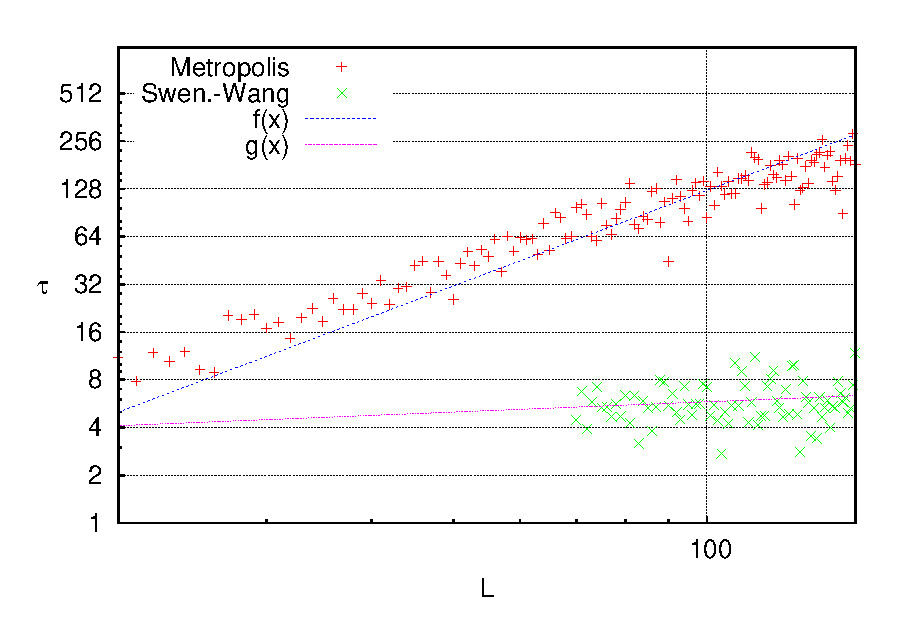
\includegraphics[scale=0.75]{Immagini/ParteB/TauHvsN}
\newline \footnotesize L=100, $K = 100000$
\end{figure}

La disposizione dei dati non è particolarmente ordinata ( era già visibile nelle figure ~\ref{fig: Cluster_CAvst} e ~\ref{fig: Metro_CAvst} l'andamento della funzione di correlazione diventa rapidamente molto rumoroso) ma è possibile dedurre dei valori approssimativi per l'esponente dinamico:
\begin{center}
\begin{tabular}{ | c | c |} 
\hline
$z_{metro}$ & $\sim$ 2 \\
\hline 
$z_{cluster}$ & $\sim$ 0.2 \\
\hline 
\end{tabular}
\end{center}

\subsection{Conclusioni}
Dalle analisi precedenti emergono le carateristiche fondamentali dei due algoritmi:
\begin{itemize}
\item \underline{Metropolis}: Soffre di una grande divergenza di $\tau_{eq}$ e del $\tau_{correlazione}$ in prossimità della $\beta$ critica. Questo comporta che per ottenere una statistica di configurazioni  significativa intorno a questa temperatura sia necessario evolvere il sistema un numero di volte molto maggiore di quanto siano i dati effettivamente ottenuti (oppure di campionare i dati dopo intervalli d'evoluzione più lunghi). 
In compenso un singolo passo dell'algoritmo richiede un tempo di esecuzione molto più basso rispetto all'algoritmo a multicluster, soprattutto per le taglie del reticolo grandi.
\item \underline{Swenden-Wang}: Il valore basso di $\tau_{correlazione}$ lo rende estremamente efficente per lo studio del sistema intorno alla temperatura critica. Anche il $\tau_{eq}$ si mantiene basso ad ogni temperatura, ciò lo rende l'algoritmo ideale per portare il sistema a termalizzazione prima di una misurazione. Il grande problema è il tempo di esecuzione e la sua forte dipendenza da $L$, infatti per simulare un sistema di taglia $L=100$ sono necessarie diverse ore. 
\end{itemize}
Per studiare i valori d'aspettazione degli osservabili macroscopici sul sistema sarà necessario sfruttare i vantaggi di entrambi gli algoritmi: l'algoritmo a multicluster verrà sfruttato per simulare la zona critica negli altri casi si farà uso dell'algoritmo di Metropolis.
\newline
Bisogna notare però che a temperature alte i due algoritmi danno valori diversi per l'osservabile di magnetizzazione assoluta( figura ~\ref{fig: Confronto_M_andamento} ).

\begin{figure}[htbp]
     \begin{minipage}{0.5\textwidth}
\centering
\caption[Preliminari$\_$Magnetizzazione.cpp ]{\footnotesize Osservabile di magnetizzazione}\label{fig: Confronto_M_andamento}
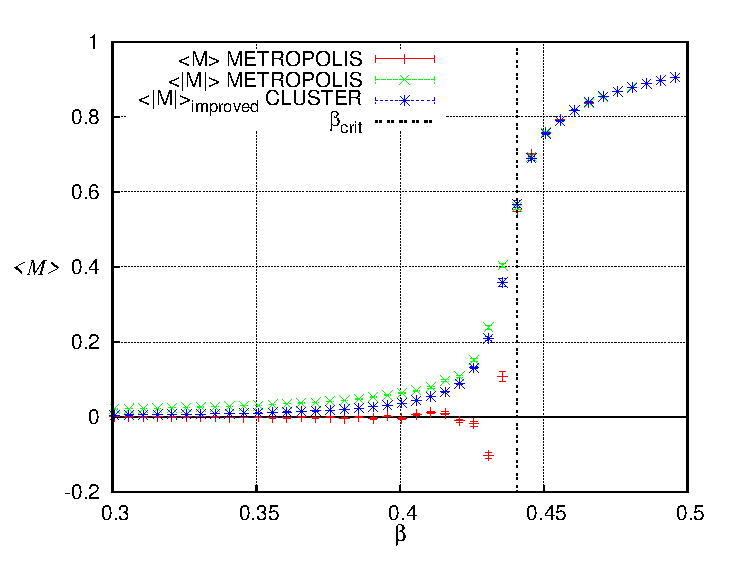
\includegraphics[scale=0.65]{Immagini/Confronto_M_andamento}
     \end{minipage}
     \begin{minipage}{0.5\textwidth}
\centering
\caption[ParteB$\_$Termal$\_$M$\_$Confronto.cpp]{\footnotesize Oscillazioni termiche }\label{fig: Confronto_M_termal}
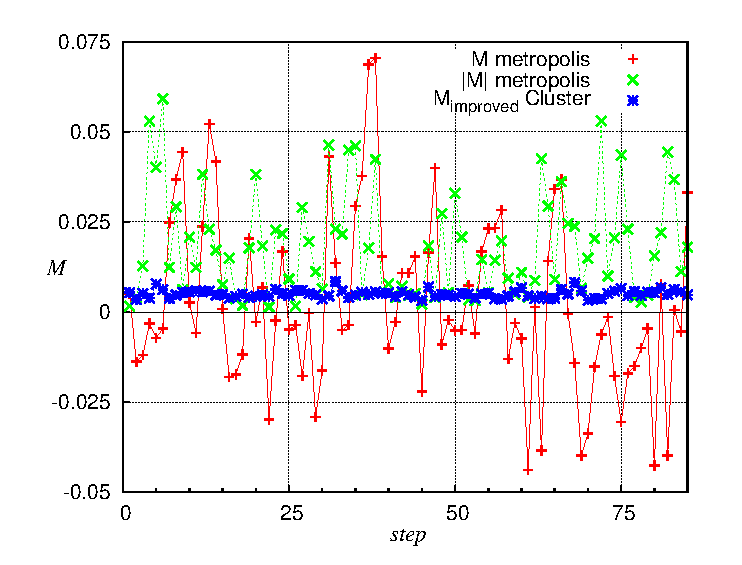
\includegraphics[scale=0.65]{Immagini/Confronto_M_termal}
     \end{minipage}
  \newline \center \footnotesize L=100, $K_{metro} = 15000$, $K_{cluster} = 1500$
\end{figure}
L'effetto è da imputare al modo differente in cui i due algoritmi simulano le fluttuazioni termiche (figura ~\ref{fig: Confronto_M_termal}).







\clearpage
\section{Comportamento Caratteristico del Modello a Taglia Finita}\label{Parte A}
A questo punto si hanno tutti gli elementi per studiare le caratteristiche del sistema di Ising attraverso la simulazione computazionale.
Ricapitolando, i principali osservabili che è possibile definire sui microstati $\phi=\lbrace \ldots, \sigma_{i\, j} ,\ldots\rbrace$ del sistema sono due:
\begin{itemize}
\item \underline{Spin Totale} $$S= \sum_{i,j=0}^{L}\sigma_{i\, j}$$
\item \underline{Energia Totale} $$ E = H(\phi) = \sum_{i,j=0}^{L}\biggr(\sigma_{i\, j}\big(\sigma_{(i+1)\, j} + \sigma_{i\, (j+1)}\big)\biggr)$$.
\end{itemize}
dove $L$ corrisponde al numero di spin in una riga, $N=L^2$ e $\sigma_{i\, j}$ e la matrice degli spin.
\newline
Le osservabili macroscopiche sono invece quattro, il loro valore d'aspettazione è da calcolare come valore medio delle "osservabili istantanee" valutate sulle singole configurazioni della catena di Markov-Montecarlo $(\phi_1,\ldots,\phi_k)$ :
\begin{itemize}
\item \underline{Magnetizzazione Media} $$\langle|M|\rangle= \langle\dfrac{|S|}{N}\rangle$$
\item \underline{Densità di Energia Interna Media} $$\langle H \rangle = \langle \dfrac{E}{N} \rangle $$
\item \underline{Calore Specifico} $$c = \beta^2 N \biggr( \langle H^2 \rangle - \langle H\rangle ^2 \biggr)$$
\item \underline{Suscettività Magnetica} $$\chi = \beta N \biggr( \langle M^2 \rangle - \langle M \rangle^2\biggr)$$
\end{itemize}
dove, per un generico osservabile istantaneo $O$ e per la generica catena $ (\phi_1, \ldots, \phi_K)$ di configurazioni campionate, vale che
\begin{displaymath}
	\langle O \rangle = \sum_{i=1}^K \dfrac{O(\phi_i)}{K}
\end{displaymath}

 \begin {figure}[h!p]
    \begin{center}
	\caption[1) ParteA\_MvsBeta.cpp \quad $/\;$ 2) ParteA\_HvsBeta.cpp ]{Magnetizzazione Assoluta e Densità di Energia}\label{fig: MvsBeta}
        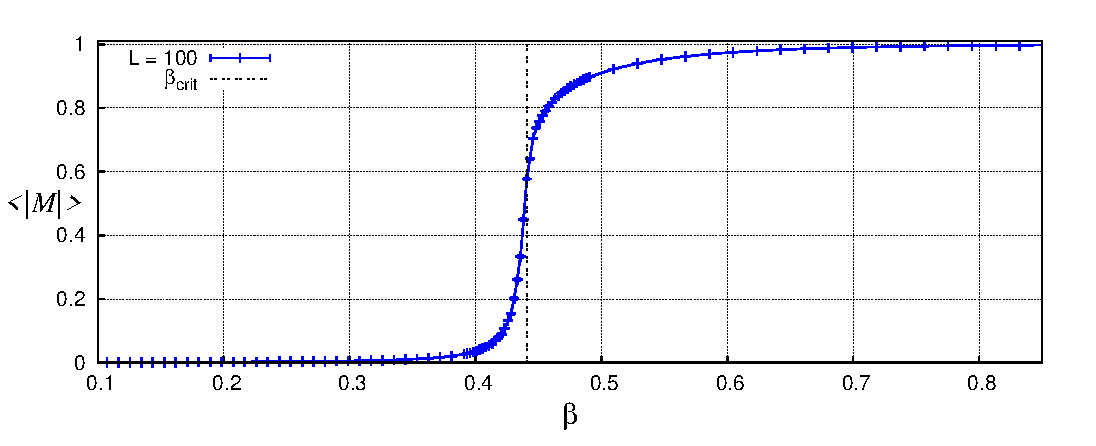
\includegraphics[scale=0.8]{Immagini/ParteA/MvsBeta}
     \newline
        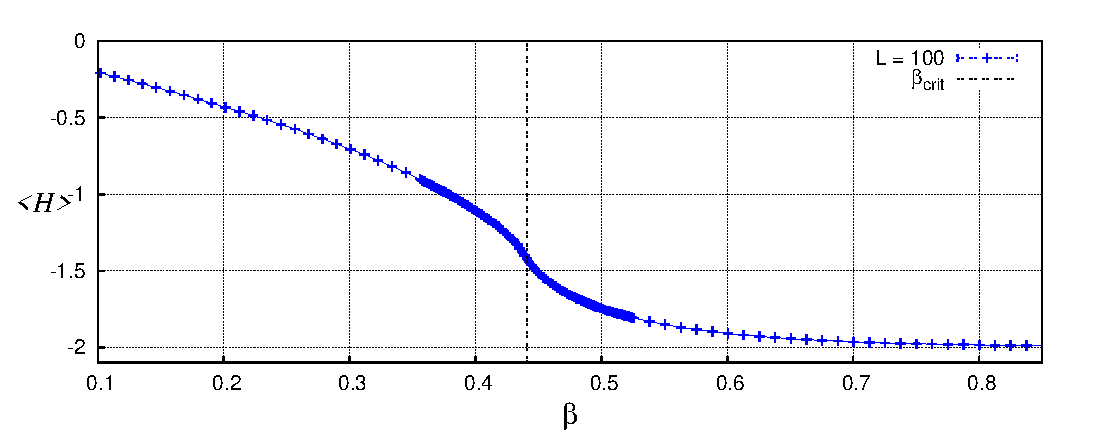
\includegraphics[scale=0.8]{Immagini/ParteA/HvsBeta}
     \newline   
	    \footnotesize L=100, $K_{metro} = 15000$, $K_{cluster} = 1500$  
    \end{center}
 \end {figure} 
 \begin {figure}[h!p]
    \begin{center}
	\caption[1) ParteA\_ChivsBeta.cpp \quad $/\;$ 2)  ParteA\_cvsBeta.cpp ]{Suscettività Magnetica e Capacità Termica}\label{fig: ChivsBeta}
        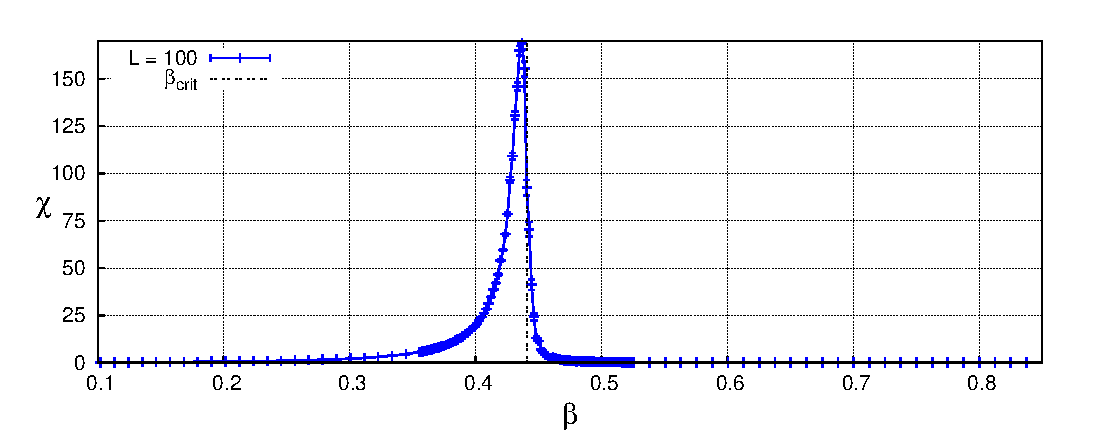
\includegraphics[scale=0.8]{Immagini/ParteA/ChivsBeta}
     \newline    
        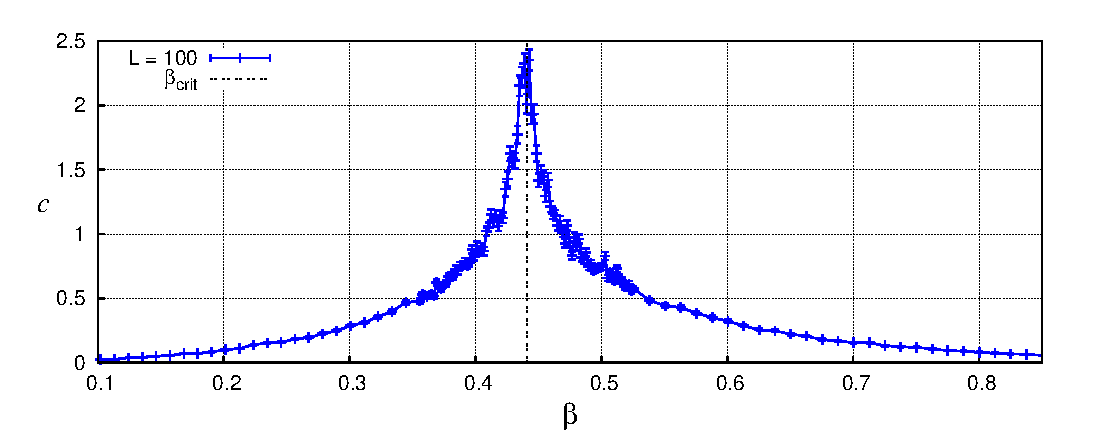
\includegraphics[scale=0.8]{Immagini/ParteA/cvsBeta}
     \newline   
		\footnotesize L=100, $K_{cluster} = 1500$  
    \end{center}
 \end {figure}

Stampando l'andamento di questi osservabili al variare della temperatura $\beta$ (figure \ref{fig: MvsBeta} e \ref{fig: ChivsBeta}) si osserva immediatamente la peculiarità del modello di Ising, ovvero la presenza di una transizione di fase attorno alla Temperatura Critica, prevista teoricamente al valore:
$$T_c =   \dfrac{\log( 1 +\sqrt{2})}{2}  = 0.44068$$
presente non sono al limite termodinamico ma anche per $L$ finito. 

\clearpage
\subsection{Calcolo dell'errore}
Le barre dell'errore nei grafici precedenti sono state calcolate tramite l'algoritmo di \emph{Jack-Knife}.
Nelle figure (\ref{fig: SigmaMvsBeta}) è mostrato l'andamento dell'incertezza per gli osservabili $M$ e $H$ calcolato tramite l'algoritmo precedente e tramite l'algoritmo di \emph{Binning} indicato per la stima dell'errore in presenza di misure correlate.

 \begin {figure}[h!]
    \begin{center}
	\caption[1) ParteA\_SigmaMvsBeta.cpp \quad $/\;$ 2) ParteA\_SigmaHvsBeta.cpp ]{Calcolo dell'incertezza sui valori d'aspettazione di $M$ e $H$ (\footnotesize vari algoritmi)}\label{fig: SigmaMvsBeta}
        \includegraphics[scale=1]{Immagini/ParteA/SigmaMvsBeta}
     \newline    
        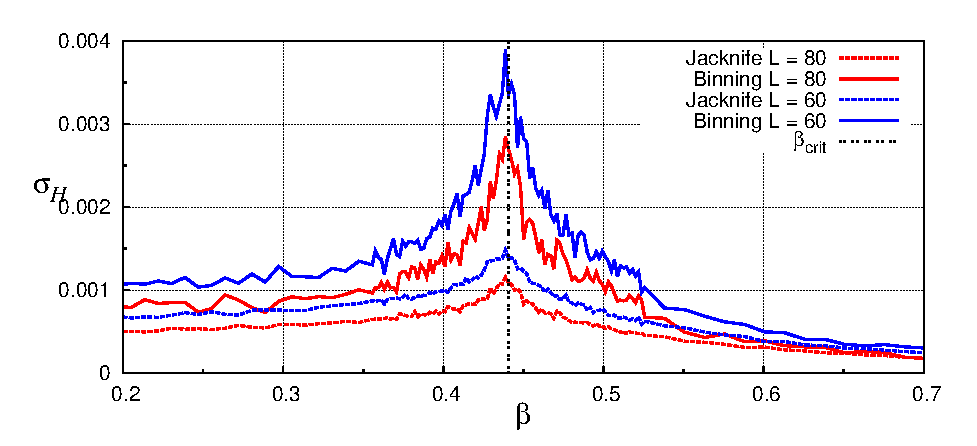
\includegraphics[scale=1]{Immagini/ParteA/SigmaHvsBeta}
     \newline   
		\footnotesize $K_{cluster} = K_{metro} = 1500$, $bin = 12$  
    \end{center}
 \end {figure}
I grafici ottenuti hanno forma simile a quelli per $\chi$ e $c$, la cosa non sorprende essendo tali osservabili legati ,  per definizione, alla varianza della magnetizzazione e dell'energia. Si nota inoltre che l'algoritmo usato porta ad una generica sottostima dell'errore rispetto al algoritmo di Binning, ma è stato scelto comunque per la maggiore semplicità di implementazione.
\newline
La crescita dell'incertezza in prossimità della temperatura critica e la sua dipendenza dalla taglia, sono l'effetto della maggiore dispersione attorno al valore medio a cui sono sottoposti gli osservabili $H$ e $M$ in queste condizioni.
 
 \begin {figure}[h!]
    \begin{center}
	\caption[1) ParteA\_distroM.cpp $\rightarrow$ distroM\_file.p \quad $/\;$ 2) ParteA\_distroH.cpp $\rightarrow$ distroH\_file.p ]{Distribuzione di probabilità sui valori d'aspettazione di $M$ e $H$ (\footnotesize vari algoritmi)}\label{fig: DistroM}
        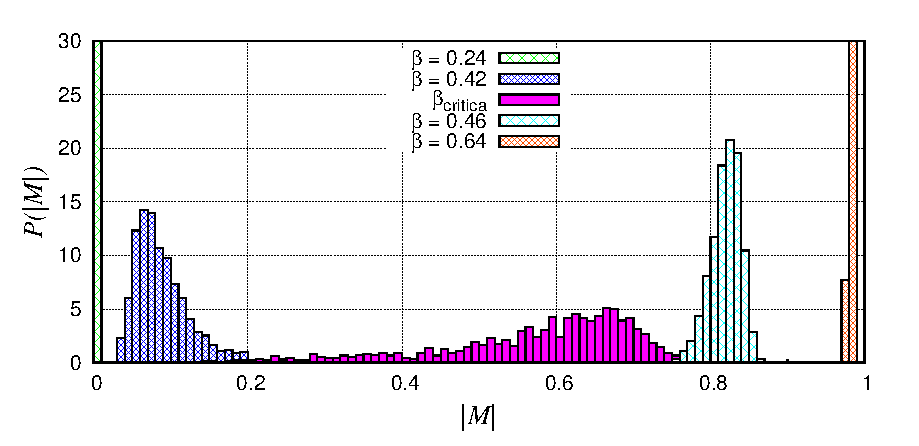
\includegraphics[scale=1]{Immagini/ParteA/distroM}
     \newline    
        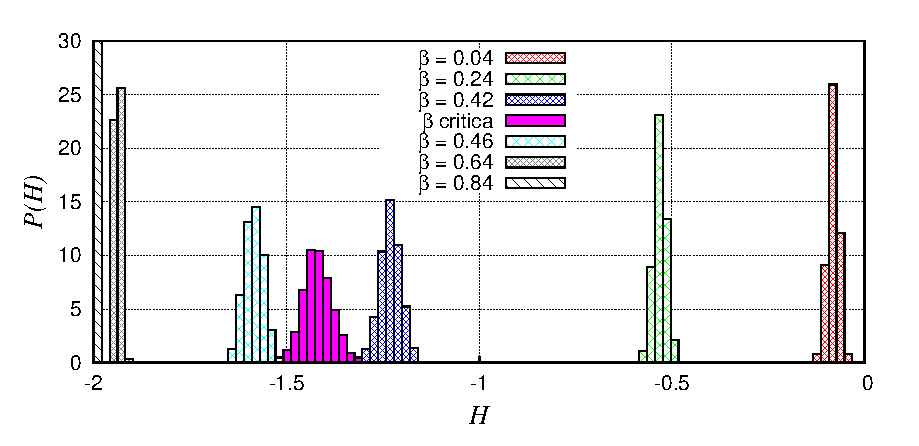
\includegraphics[scale=1]{Immagini/ParteA/distroH}
     \newline   
		\footnotesize $K_{cluster}$ \newline(nb: Nel grafico il range dell'asse è tagliato per rendere più visibili le distribuzioni vicino a $T_c$, lontano da $T_c$ le distribuzioni sono piccate in una sola colonna).   
    \end{center}
 \end {figure}
A prova di questo nelle figura \ref{fig: DistroM} sono mostrate le distribuzioni di probabilità( istogrammi normallizati) dei valori di $H$ e $M$ per differenti temperature di termalizzazione.
\clearpage
\section{Studio della Lunghezza di Autocorrelazione}\label{Parte C}
\begin{wrapfigure}{r}{0.3\textwidth}
\vspace{-25pt} 
  \begin{center}
	\includegraphics[width=0.28\textwidth]{Immagini/Reticolo}
  \end{center}
       \vspace{-15pt} 
       \caption[Campionatura per la Funzione di Correlazione.]{\footnotesize Campionatura per la Funzione di Correlazione.}\label{fig: simmetrie}
       \vspace{-15pt} 
\end{wrapfigure}

Per correlazione si intende una relazione tra variabili casuali tale per cui a ciascun valore assunto dalla prima variabile corrisponde, con una certa probabilità, un valore della seconda.
Nel capitolo \ref{Parte B} è già stata introdotta una misura di correlazione, il tempo di autocorrelazione $\tau$, che misura la similitudine delle osservabili microscopiche tra due configurazioni campionate a tempo diverso.

In questo capitolo verrà studiata un'altra misura di correlazione, le variabili prese in considerazione saranno la coppia $S_0$, spin medio su una  generica riga del reticolo e $S_t$, spin medio su una seconda riga posta a $t$ passi reticolari dalla riga scelta. 
Lo scopo di questa analisi è di stimare fino a quale distanza lo spin in un punto riesce ad influenzare lo stato di un'altro nodo del sistema, questo tipo di interazione è totalmente indiretta visto che l'Hamiltoniana prevede solo interazioni tra siti primi vicini.

Per quantificare la correlazione tra righe diverse è necessario introdurre una funzione di correlazione, definita in modo simile alla funzione precedente:

\begin{equation}\label{eq: G_c}
G_c(t) = \dfrac{\langle S_i S_{i+t}\rangle - \langle S_i\rangle \langle S_{i+t}\rangle  }{\langle S_i^2\rangle - \langle S_i\rangle \langle S_{i}\rangle} \simeq \dfrac{\langle S_i S_{i+t}\rangle}{\langle S_i^2\rangle}
\end{equation}
dove le medie vanno intese come medie su tutti i valori campionati dello spin medio su una riga.

Per via delle simmetrie rotazionali ( di $90^\circ$) e traslazionali ( di passi reticolari) del reticolo quadrato, per ogni configurazione simulata si avranno $2L$ coppie di misure su cui valutare la correlazione.
L'ultima uguglianza nell'equazione \ref{eq: G_c} è un'approssimazione valida per le temperature $T>Tc$ dove, teoricamente, la magnetizzazione è nulla. 

In questo caso la funzione di correlazione quantifica la probabilità che due righe poste a $t$ passi di distanza abbiano lo stesso valore di magnetizzazione, infatti quando le coppie di righe hanno lo stesso spin $G_c = 1$ invece quando le magnetizzazioni tendono ad essere discordi e concordi con la medesima probabilità si avrà $G_c \rightarrow 0 $.
\medskip

Esattamente come nel caso dell'autocorrelazione si attende che la funzione di correlazione tra righe decada esponenzialmente:
\begin{equation}
G_c(t) \simeq e^{-t/\xi}
\end{equation}
dove il coefficiente $\xi$ del decadimento viene chiamato \emph{lunghezza di correlazione}.
Ovviamente anche in questo caso $\xi$ equivale al valore di $t$ per cui la correlazione corrisponde ad $e^-1$, quindi la quantità $2 \xi$ è la distanza dopo cui due linee possono essere considerate scorrelate.
\begin{figure}[h!]
   \caption[ParteC$\_$StS0vst$\_$Cluster.cpp ]{Andamento del coefficiente di correlazione medio tra coppie di linee in funzione della distanza $t$ per vari valori di $\beta$.}\label{fig: Cluster_S0Stvst}
     \centering
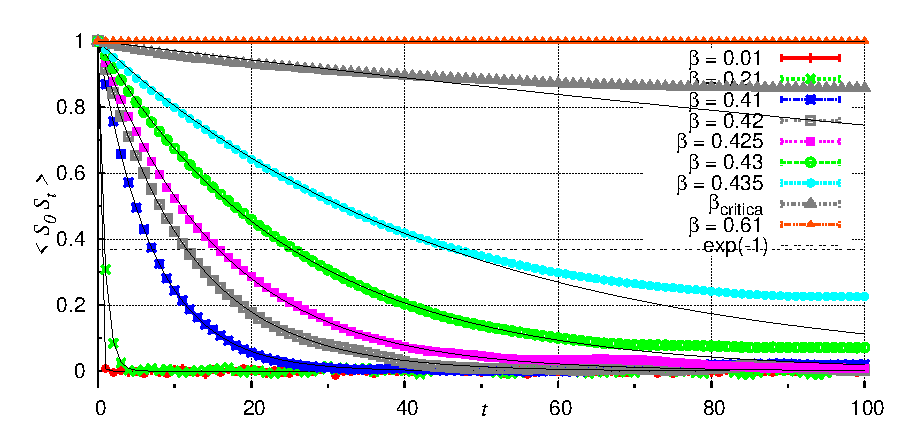
\includegraphics[width=1\textwidth]{Immagini/ParteC/Cluster_S0Stvst}
\end{figure}


\bigskip
Nella figura (\ref{fig: Cluster_S0Stvst}) è mostrato l'andamento della funzione di correlazione per uno stesso sistema simulato a $\beta$ crescenti fino al raggiungimento della temperatura critica (in questo intervallo è possibile usare l'espressione approssimata di $G_c$) dopo la fase critica il sistema è completamente magnetizzato, la maggior parte degli spin sono paralleli, e quindi il sistema risultarà sempre completamente correlato.
A ciascun set di dati è sovrapposto il fit esponenziale eseguito unicamente sui primi punti in modo da poter ignorare il comportamento rumoroso presente per alti valori di $t$.

Si noti come l'accordo con l'andamento esponenziale diminuisca al tendere di $\beta$ a $\beta_c$, l'effetto è dovuto al fatto che i modelli ad $L$ finito presentano una magnetizzazione residua anche alla temperatura critica laddove la soluzione teorica di Onsanger prevederebbe una magnetizzazione esattamente nulla(per tutte le temperature maggiori del valore critico).
\newline
Dal grafico è evidente come la lunghezza di correlazione, parametro $\xi$ che regola la concavità della funzione, cresca man mano che la temperatura diminuisce, dai fit esponenziali si ottengono le seguenti stime della lunghezza di correlazione:

\begin{center}
\begin{tabular}{|c|c |r c l| }
\hline
$\beta$	& $\xi$ \footnotesize{"ad occhio"}	&\multicolumn{3}{|c|}{$\xi_{fit}$	} \\
0,01	& $\sim$ 0,5	&0,20	&$\pm$	&0,01\\
0,21	& $\sim$ 1	&0,84	&$\pm$	&0,01\\
0,41	& $\sim$ 7	&7,11	&$\pm$	&0,02\\
0,42	& $\sim$ 11,5	&11,65	&$\pm$	&0,02\\
0,425	& $\sim$ 16	&15,75	&$\pm$	&0,04\\
0,43	& $\sim$ 25,5	&25,37	&$\pm$	&0,04\\
0,435	& $\sim$ 43,5	&45,79	&$\pm$	&0,11\\
critico	& oltre 100	&340,20	&$\pm$	&7,3\\
\hline
0,61	& $\infty$ 	& 	& $\infty$	& \\
\hline
\end{tabular}
\end{center}

Eseguendo questo stesso procedimento su una raccolta di dati più vasta( 80 valori di $\beta < \beta_c$) si può ottenere un grafico di $\xi$ in funzione di $X=\small \dfrac{\beta -\beta_c}{\beta_c}$( figura \ref{fig: XivsBeta}).

\begin{figure}[h!]
       \caption[ParteC$\_$StS0vst$\_$Moltitudini $\;\rightarrow\;$ molti\_S0Stvst.p ]{Andmaneto della lunghezza di correlazione in funzione della temperatura del sistema.}\label{fig: Xivst}
     \centering
		\includegraphics[width=0.70\textwidth]{Immagini/ParteC/xivst}

\footnotesize  $L= 200$ , $N_{configurazioni} = 100$
\end{figure}

Dal grafico è evidente come il valore della lunghezza di correlazione diverga molto velocemente avvicinandosi alla temperatura critica.
L'andamento ha tendenzialmente un buon accordo con $1/X$ fino al valore critico dove, in conseguenza alla dimensione finita del reticolo, la divergenza è limitata ad un valore massimo $\xi_L(\beta_c)$ grande ma finito.

\subsubsection*{Dipendenza di $\xi_L(\beta_c)$ da L}
Resta da determinare come il valore massimo $\xi_L(\beta_c)$ dipenda dalla dimensione del reticolo.
Per farlo si simulano vari sistemi con differente taglia del reticolo e si studia l'andamento della funzione di correlazione $G_c$ (approssimata) alla temperatura critica ( figura: \ref{fig: Cluster_Tc_S0Stvst} ).
Purtroppo l'accordo dell'espressione approssimata della funzione di correlazione con l'andamento esponenziale è molto debole a questa temperatura, si può comunque eseguire un fit esponenziale sui primi valori dei dati campionati ottenendo i seguenti valori:


     \begin{minipage}{0.3\textwidth}
		\begin{tabular}{|c|r c l| }
			\hline \footnotesize
			$\beta$	&\multicolumn{3}{|c|}{$\xi_{fit}$	} \\
330	&515,6	&$\pm$	&11,6\\
320	&384,7	&$\pm$	&6\\
310	&385,7	&$\pm$	&7,3\\
300	&278,69	&$\pm$	&4,5\\
290	&346,53	&$\pm$	& 7,5\\
280	&324,267	&$\pm$	& 6,6\\
270	&409,24	&$\pm$	& 10,51\\
260	&317,69	&$\pm$	& 6,8\\
250	&323,06	&$\pm$	& 6,5\\
240	&311,43	&$\pm$	& 7,1\\

\hline
\end{tabular}
     \end{minipage}\hfill
     \begin{minipage}{0.3\textwidth}
\begin{tabular}{|c|r c l| }
\hline \footnotesize
$\beta$	&\multicolumn{3}{|c|}{$\xi_{fit}$	} \\
230	&260,34	&$\pm$	& 4,864\\
220	&215,09	&$\pm$	& 3,23\\
210	&245,38	&$\pm$	& 4,69\\
200	&211,84	&$\pm$	& 3,43\\
190	&258,95	&$\pm$	& 5,76\\
180	&242,76	&$\pm$	& 6,12\\
170	&157	&$\pm$	& 1,98\\
160	&234,79	&$\pm$	& 5,31\\
150	&216,71	&$\pm$	& 5,36\\
140	&191,01	&$\pm$	& 4,21\\

\hline
\end{tabular}
     \end{minipage}\hfill
     \begin{minipage}{0.3\textwidth}
\begin{tabular}{|c|r c l| }
\hline \footnotesize
$\beta$	&\multicolumn{3}{|c|}{$\xi_{fit}$	} \\
130	&198,53	&$\pm$	& 4,95\\
120	&160,1	&$\pm$	& 3,55\\
110	&234	&$\pm$	& 8,88\\
100	&175,4	&$\pm$	& 4,63\\
90	&133,66	&$\pm$	& 3,79\\
80	&114,16	&$\pm$	& 2,81\\
70	&90,6	&$\pm$	& 2,43\\
60	&164,1	&$\pm$	& 8,22\\
50	&148,1	&$\pm$	& 7,44\\
40	&106,53	&$\pm$	& 5,66\\
\hline
\end{tabular}
     \end{minipage}\hfill

\begin{figure}[htbp]
      \centering
      \caption[ParteC\_Tc\_StS0vst\_Cluster.cpp ]{Andamento della funzione di Correlazione in funzione della distanza $t$ alla temperatura critica.}\label{fig: Cluster_Tc_S0Stvst}
	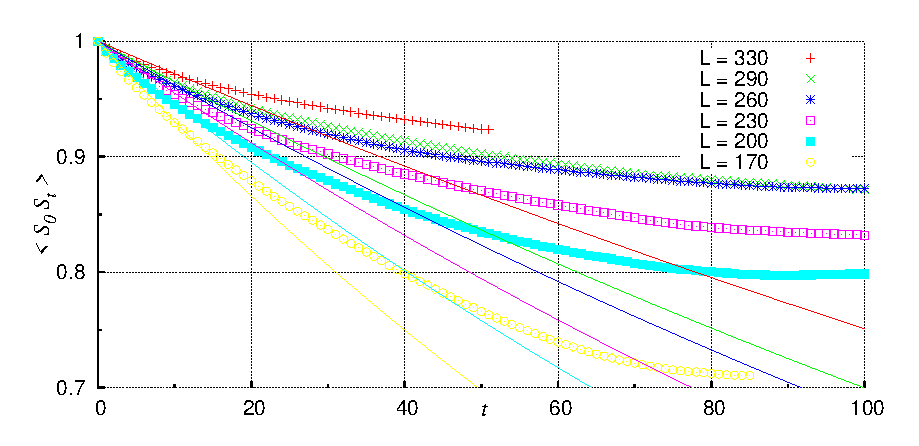
\includegraphics[width=1\textwidth]{Immagini/ParteC/Cluster_Tc_S0Stvst}
	\bigskip
	  \caption[ParteC\_Tc\_StS0vst\_Cluster.cpp $\;\rightarrow\;$ grafico\_file.p ]{Andamento della lunghezza di correlazione calcolata tramite il fit esponenziale dei grafici precedenti in funzione della taglia $L$.}\label{fig: grafpo_Tc}
	\includegraphics[width=1\textwidth]{Immagini/ParteC/grafpo_Tc}
\end{figure}
La dipendenza dei dati campionati di $\xi_L(\beta_c)$ da $L$ (figura \ref{fig: grafpo_Tc}) non è particolarmente regolare, ma si può notare (figure \ref{fig: Cluster_Tc_S0Stvst} e \ref{fig: grafpo_Tc}) come l'andamento sia distribuito in modo approsimativamente uniforme intorno ad una retta.
Si può concludere quindi che :
$$\xi_L(\beta_c) \simeq L $$


\clearpage
\section{Studio di Finite Size Scaling}\label{Parte D}
A livello teorico è previsto un andamento della \emph{lunghezza di correlazione} in prossimità della temperatura critica del tipo:
\begin{equation}\label{eq: xivst}
\xi \propto \big| \dfrac{T - T_c}{T_c} \big|^{(-\nu)} = |t|^{(-\nu)}
\end{equation}
dove è stato introdotto il fattore $\nu$, detto \emph{esponenete critico}, che regola la divergenza ed è stimato essere  $\nu = 1$.

Ammettendo che sia la divergenza della lunghezza di correlazione a determinare il comportamento critico delle altre osservabili intorno a $T_c$ si potranno definire per tali quantità espressioni dello simili all' equazione (\ref{eq: xivst}) :

\begin{eqnarray}\label{eq: criticexpo}
 c & \propto & |t|^{-\alpha}  \propto \xi^{-\alpha / \nu}       \nonumber \\
 |M|  & \propto & \propto \xi^{-\beta / \nu}  \qquad (\textrm{\footnotesize{ solo per $T < T_c$}})\\
 \chi & \propto & |t|^{-\gamma}  \propto \xi^{-\gamma / \nu}
\end{eqnarray}

Il valore di questi esponenti critici non è stimabile in modo diretto ( attraverso un fit su punti campionati tramite delle simulazioni ad esempio) per via del vincolo della taglia finita che sta alla base di qualsiasi simulazione computazionale.
Non ci si aspetta che tale vincolo determini un generico cambiamento della dipendenza di $xi$ da $\beta$ ma che intervanga solamente causando un "cut-off" della divergenza della lunghezza di correlazione in prossimità alla temperatura critica.
Per un reticolo finito qualsiasi distanza non potrà essere maggiore della dimensione caratterisitica del sistema data dal lato del reticolo( la taglia $L$)\footnote{In realtà in presenza della condizione di bordo periodico la distanza massima che può essere sottesa tra due punti sarà $L/\sqrt{2}$}. Pertanto risulterà che:
\begin{equation}\label{eq: Xi_l}
\xi_L = \left\{ \begin{array}{rl}
 \xi_{\mbox{teo}}  &\mbox{ se $t \neq 0$} \\
  L &\mbox{ se $t \simeq 0$}
       \end{array} \right.
\end{equation}
\bigskip

Un criterio per stimare gli esponenti critici viene fornito dal metodo di \emph{Finite Size Scaling}.
Questa tecnica si basa sullo studio dell'andamento delle quantità osservabili in funzione della taglia $L$.
L'idea è la seguente: si consideri un osservabile critico, $\chi$ ad esempio, teoricamente la divergenza del valore d'aspettazione dipende dalla divergenza della lunghezza di correlazione secondo l'equazione \ref{eq: criticexpo} ma in un modello a taglia finita l'andamento di $\xi$ è limitato in accordo con l'equazione \ref{eq: Xi_l}. 
Unendo le due equazioni precedenti si ottiene il comportamento complessivo dell'osservabile $\chi$ per un sistema finito:
\begin{equation}\label{eq: Chi_finite}
\chi = \xi^{\gamma /\nu} \chi_0 (L/\xi)
\end{equation}
Nell'equazione è stata introdotta la funzione adimensionale $\chi_0:\mathbb{R} \rightarrow \mathbb{R}$ definita come:
\begin{equation}
\chi_0 (x) \propto \left\{ \begin{array}{rl}
		\mbox{cost}  &\mbox{ se $x \gg 1$} \\
  x^{-\gamma/\nu} &\mbox{ se $x \rightarrow 0$} \\
       \end{array} \right.
\end{equation}
la cui forma funzionale (incognita) rappresenta il modo esatto in cui il valore della suscettività viene smorzato per temperature vicino a $T_c$. 
La funzione è costruita in modo da non contere alcuna dipendenza implicita da $\xi$ che appare unicamente all'interno dell' argomento.

La dipendenza dalla lunghezza di correlazione può essere nascosta definendo una nuova funzione, detta \emph{di scaling},
\begin{equation}
\tilde{\chi}(x) = x^{-\gamma}\chi_0(x^{v}) \propto \left\{ \begin{array}{rl}
		x^{-\gamma}  &\mbox{ se $x \gg 1$} \\
  \mbox{cost} &\mbox{ se $x \rightarrow 0$} \\
       \end{array} \right.
\end{equation}
per cui risulta l'equazione:
\begin{equation}
\chi = L^{\gamma / \nu} \tilde{\chi}(L^{1/\nu} |t|)
\end{equation}
che descrive il modo in cui il valore di suscettività attorno alla temperatura critica varia in funzione di $L$.

\medskip
L'andamento preciso della funzione di scaling appena introdotta è incognito, ma per costruzione presenta due importanti proprietà:
\begin{itemize}
\item[-] La funzione di scaling è costante alla temperatura critica: 
		\begin{displaymath}
			\tilde{\chi}(x) \xrightarrow[x\rightarrow 0]{} x^{-\gamma}(x^\nu)^{\gamma/\nu} = \mbox{cost}
		\end{displaymath}
\item[-] La forma funzionale di $\tilde{\chi}$ non dipende da $L$. Pertanto il valore nell'origine ($T = T_c$) oltre ad essere costante è lo stesso per ogni sistema simulato a $L$ finito.
\end{itemize}

\medskip
Tutto questo può essere sfruttato per determinare gli esponenti critici: per prima cosa si campionano un buon numero di valori d'aspettazione degli osservabili critici ($\chi_L(t)$ , $c_L(t)$ e $M_L(t)$) intorno alla temperatura critica e per varie taglie $L$ finite. Per ciascuno di tali osservabili varrà la relazione:

\begin{displaymath}
	\tilde{O}(L^{1/ \nu} t ) = L^{\theta / \nu}O_L(t)
\end{displaymath}
(dove $\theta$ è l'esponente critico associato all'osservabile O).
Per ogni osservabile è possibile costruire un grafico ponendo come ascissa il valore $x = L^{1/ \nu} t $ e come ordinata
$y = L^{\theta / \nu}O_L(t)$. 
Questo grafico rappresenterà l'andamento della funzione di scaling incognita a condizione che gli esponenti $ \theta $ e $ \nu $ verranno scelti esattamente coincidenti al valore dell'esponente critico.
Confrontando i grafici a differente $L$ relativi allo stesso osservabile si può dare una stima degli esponenti critici come valori per cui tutti gli andamenti collassano alla medesima curva universale, caratteristica dell'osservabile preso in considerazione.
\medskip \newline
La stima degli esponenti critici è stata ottenuta ponendo i dati campionati in un foglio di calcolo\footnote{File: \emph{Finite Size Scaling.xls}} e osservando come cambia la forma dei grafici al variare degli esponenti $\theta$ e $\nu$. I valori per cui tutti i grafici collassano approssimativamente ad una sola curva costituisco una stima per gli esponenti critici.
Da questa analisi risultano i seguenti risultati:
\begin{center}
\begin{tabular}{|c|c|}
\hline
	$ \nu $ &= 1 $\pm$ 0,1 \\
\hline
	$ \alpha $ &= 0,1 $\pm$ 0,2 \\
\hline
	$ \beta $ &= 1,25 $\pm$ 0,02 \\
\hline
	$ \gamma $ &= 1,75 $\pm$ 0,01 \\
\hline
\end{tabular}
\end{center}
(l'errore è calcolato in modo qualitativo stimando l'intervallo di valori in cui l'accordo con la curva universale appare ottimale).
Nelle figure (\ref{fig: Chi_finitesize_1}), (\ref{fig: M_finitesize_1}) e (\ref{fig: c_finitesize_1}) è mostrato il confronto tra gli andamenti originali degli osservabili critici (in funzione di $t= (T-T_c) / T_c$) a varie taglie e la curva ottenuta tramite l'analisi di Finite Size che ha condotto alle stime precedenti.


\begin{figure}[htbp]
      \centering
      \caption[ParteD\_Ossvst.cpp $\;\rightarrow\;$ Chivst\_file.p ]{Studio di Finite Size Scaling dell'osservabile $\chi$.}\label{fig: Chi_finitesize_1}
	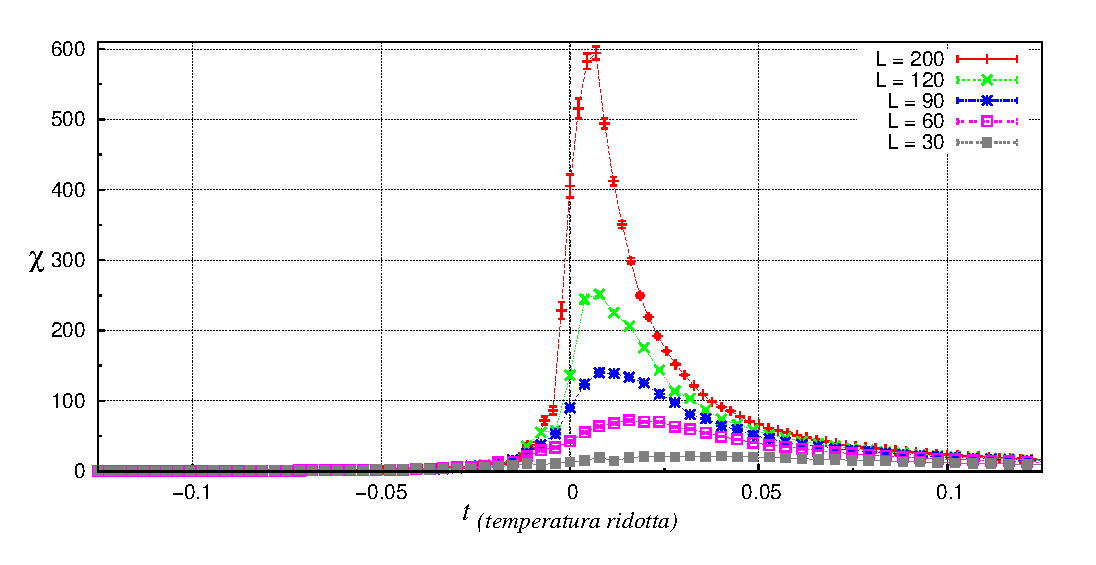
\includegraphics[width=1\textwidth]{Immagini/ParteD/Chivst}
	\bigskip
%	  \caption{}\label{fig: Chi_finitesize_2}
	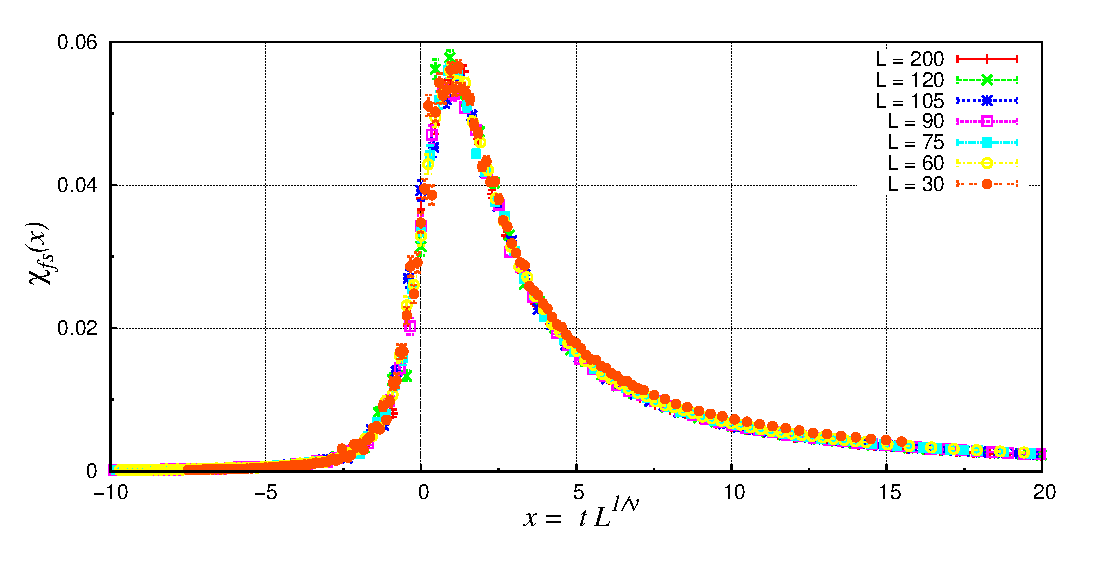
\includegraphics[width=1\textwidth]{Immagini/ParteD/Chivst_finite}
\end{figure}

\begin{figure}[htbp]
      \centering
      \caption[ParteD\_Ossvst.cpp $\;\rightarrow\;$ Mvst\_file.p ]{Studio di Finite Size Scaling dell'osservabile $M$.}\label{fig: M_finitesize_1}
	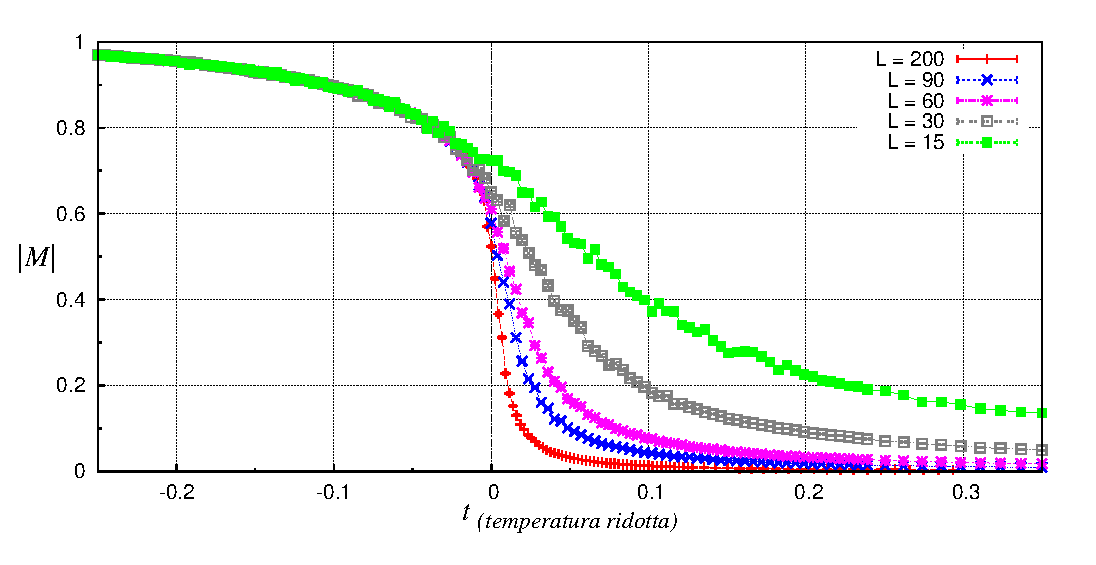
\includegraphics[width=1\textwidth]{Immagini/ParteD/Mvst}
	\bigskip
%	  \caption{}\label{fig: M_finitesize_2}
	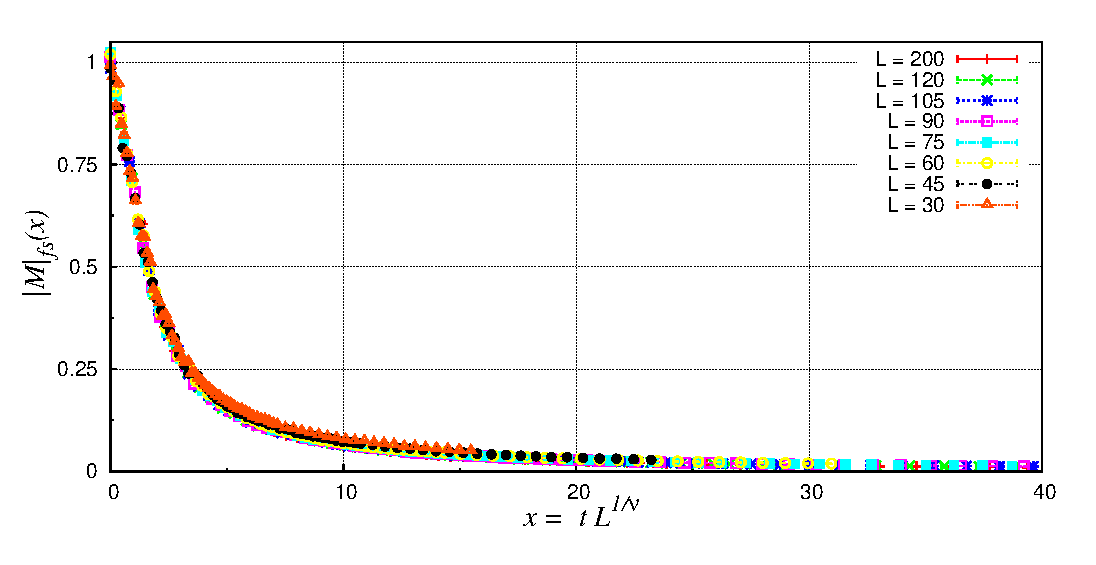
\includegraphics[width=1\textwidth]{Immagini/ParteD/Mvst_finite}
\end{figure}

\begin{figure}[htbp]
      \centering
      \caption[ParteD\_Ossvst.cpp $\;\rightarrow\;$ cvst\_file.p ]{Studio di Finite Size Scaling dell'osservabile $c$.}\label{fig: c_finitesize_1}
	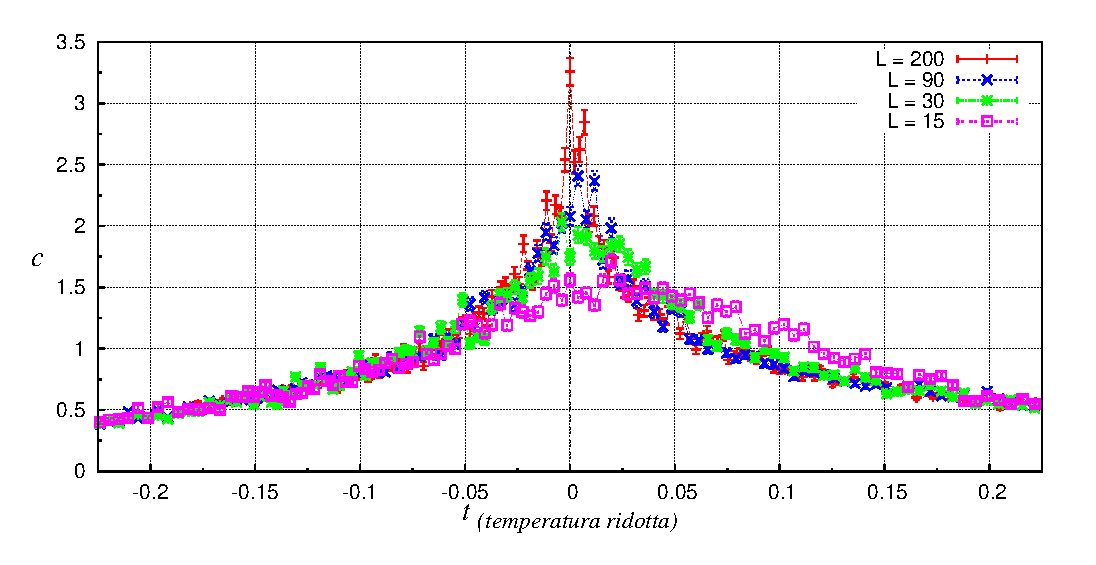
\includegraphics[width=1\textwidth]{Immagini/ParteD/cvst}
	\bigskip
%	  \caption{}\label{fig: c_finitesize_2}
	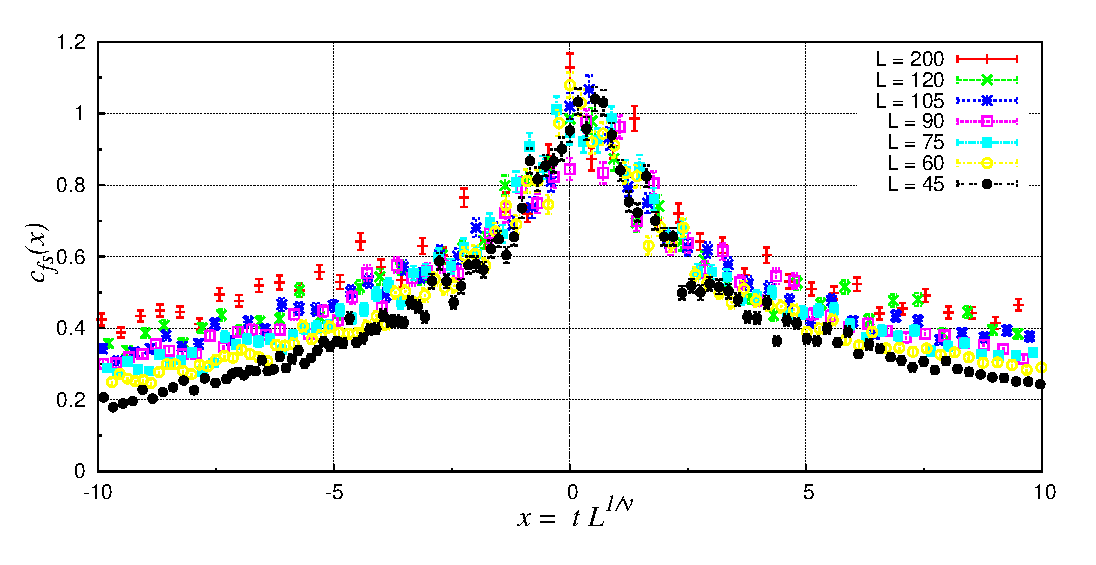
\includegraphics[width=1\textwidth]{Immagini/ParteD/cvst_finite}
\end{figure}






\clearpage
\listoffigures

\bibliographystyle{plain}
\bibliography{Bibi.bib}


\end{document}
This is never printed


classi \Cls{Nomeclasse}

metodi \cd{NomeMetodo}

tipo \cd{Nometipo}
